% Options for packages loaded elsewhere
\PassOptionsToPackage{unicode}{hyperref}
\PassOptionsToPackage{hyphens}{url}
\PassOptionsToPackage{dvipsnames,svgnames*,x11names*}{xcolor}
%
\documentclass[
  12pt, krantz2,
]{book}
\usepackage{lmodern}
\usepackage{amssymb,amsmath}
\usepackage{ifxetex,ifluatex}
\ifnum 0\ifxetex 1\fi\ifluatex 1\fi=0 % if pdftex
  \usepackage[T1]{fontenc}
  \usepackage[utf8]{inputenc}
  \usepackage{textcomp} % provide euro and other symbols
\else % if luatex or xetex
  \usepackage{unicode-math}
  \defaultfontfeatures{Scale=MatchLowercase}
  \defaultfontfeatures[\rmfamily]{Ligatures=TeX,Scale=1}
\fi
% Use upquote if available, for straight quotes in verbatim environments
\IfFileExists{upquote.sty}{\usepackage{upquote}}{}
\IfFileExists{microtype.sty}{% use microtype if available
  \usepackage[]{microtype}
  \UseMicrotypeSet[protrusion]{basicmath} % disable protrusion for tt fonts
}{}
\makeatletter
\@ifundefined{KOMAClassName}{% if non-KOMA class
  \IfFileExists{parskip.sty}{%
    \usepackage{parskip}
  }{% else
    \setlength{\parindent}{0pt}
    \setlength{\parskip}{6pt plus 2pt minus 1pt}}
}{% if KOMA class
  \KOMAoptions{parskip=half}}
\makeatother
\usepackage{xcolor}
\IfFileExists{xurl.sty}{\usepackage{xurl}}{} % add URL line breaks if available
\IfFileExists{bookmark.sty}{\usepackage{bookmark}}{\usepackage{hyperref}}
\hypersetup{
  pdftitle={{[}SER 2021 Workshop{]} Causal Mediation: Modern Methods for Path Analysis},
  pdfauthor={Iván Díaz, Nima Hejazi, Kara Rudolph},
  colorlinks=true,
  linkcolor=Maroon,
  filecolor=Maroon,
  citecolor=Blue,
  urlcolor=Blue,
  pdfcreator={LaTeX via pandoc}}
\urlstyle{same} % disable monospaced font for URLs
\usepackage{color}
\usepackage{fancyvrb}
\newcommand{\VerbBar}{|}
\newcommand{\VERB}{\Verb[commandchars=\\\{\}]}
\DefineVerbatimEnvironment{Highlighting}{Verbatim}{commandchars=\\\{\}}
% Add ',fontsize=\small' for more characters per line
\usepackage{framed}
\definecolor{shadecolor}{RGB}{248,248,248}
\newenvironment{Shaded}{\begin{snugshade}}{\end{snugshade}}
\newcommand{\AlertTok}[1]{\textcolor[rgb]{0.94,0.16,0.16}{#1}}
\newcommand{\AnnotationTok}[1]{\textcolor[rgb]{0.56,0.35,0.01}{\textbf{\textit{#1}}}}
\newcommand{\AttributeTok}[1]{\textcolor[rgb]{0.77,0.63,0.00}{#1}}
\newcommand{\BaseNTok}[1]{\textcolor[rgb]{0.00,0.00,0.81}{#1}}
\newcommand{\BuiltInTok}[1]{#1}
\newcommand{\CharTok}[1]{\textcolor[rgb]{0.31,0.60,0.02}{#1}}
\newcommand{\CommentTok}[1]{\textcolor[rgb]{0.56,0.35,0.01}{\textit{#1}}}
\newcommand{\CommentVarTok}[1]{\textcolor[rgb]{0.56,0.35,0.01}{\textbf{\textit{#1}}}}
\newcommand{\ConstantTok}[1]{\textcolor[rgb]{0.00,0.00,0.00}{#1}}
\newcommand{\ControlFlowTok}[1]{\textcolor[rgb]{0.13,0.29,0.53}{\textbf{#1}}}
\newcommand{\DataTypeTok}[1]{\textcolor[rgb]{0.13,0.29,0.53}{#1}}
\newcommand{\DecValTok}[1]{\textcolor[rgb]{0.00,0.00,0.81}{#1}}
\newcommand{\DocumentationTok}[1]{\textcolor[rgb]{0.56,0.35,0.01}{\textbf{\textit{#1}}}}
\newcommand{\ErrorTok}[1]{\textcolor[rgb]{0.64,0.00,0.00}{\textbf{#1}}}
\newcommand{\ExtensionTok}[1]{#1}
\newcommand{\FloatTok}[1]{\textcolor[rgb]{0.00,0.00,0.81}{#1}}
\newcommand{\FunctionTok}[1]{\textcolor[rgb]{0.00,0.00,0.00}{#1}}
\newcommand{\ImportTok}[1]{#1}
\newcommand{\InformationTok}[1]{\textcolor[rgb]{0.56,0.35,0.01}{\textbf{\textit{#1}}}}
\newcommand{\KeywordTok}[1]{\textcolor[rgb]{0.13,0.29,0.53}{\textbf{#1}}}
\newcommand{\NormalTok}[1]{#1}
\newcommand{\OperatorTok}[1]{\textcolor[rgb]{0.81,0.36,0.00}{\textbf{#1}}}
\newcommand{\OtherTok}[1]{\textcolor[rgb]{0.56,0.35,0.01}{#1}}
\newcommand{\PreprocessorTok}[1]{\textcolor[rgb]{0.56,0.35,0.01}{\textit{#1}}}
\newcommand{\RegionMarkerTok}[1]{#1}
\newcommand{\SpecialCharTok}[1]{\textcolor[rgb]{0.00,0.00,0.00}{#1}}
\newcommand{\SpecialStringTok}[1]{\textcolor[rgb]{0.31,0.60,0.02}{#1}}
\newcommand{\StringTok}[1]{\textcolor[rgb]{0.31,0.60,0.02}{#1}}
\newcommand{\VariableTok}[1]{\textcolor[rgb]{0.00,0.00,0.00}{#1}}
\newcommand{\VerbatimStringTok}[1]{\textcolor[rgb]{0.31,0.60,0.02}{#1}}
\newcommand{\WarningTok}[1]{\textcolor[rgb]{0.56,0.35,0.01}{\textbf{\textit{#1}}}}
\usepackage{longtable,booktabs}
% Correct order of tables after \paragraph or \subparagraph
\usepackage{etoolbox}
\makeatletter
\patchcmd\longtable{\par}{\if@noskipsec\mbox{}\fi\par}{}{}
\makeatother
% Allow footnotes in longtable head/foot
\IfFileExists{footnotehyper.sty}{\usepackage{footnotehyper}}{\usepackage{footnote}}
\makesavenoteenv{longtable}
\usepackage{graphicx,grffile}
\makeatletter
\def\maxwidth{\ifdim\Gin@nat@width>\linewidth\linewidth\else\Gin@nat@width\fi}
\def\maxheight{\ifdim\Gin@nat@height>\textheight\textheight\else\Gin@nat@height\fi}
\makeatother
% Scale images if necessary, so that they will not overflow the page
% margins by default, and it is still possible to overwrite the defaults
% using explicit options in \includegraphics[width, height, ...]{}
\setkeys{Gin}{width=\maxwidth,height=\maxheight,keepaspectratio}
% Set default figure placement to htbp
\makeatletter
\def\fps@figure{htbp}
\makeatother
\setlength{\emergencystretch}{3em} % prevent overfull lines
\providecommand{\tightlist}{%
  \setlength{\itemsep}{0pt}\setlength{\parskip}{0pt}}
\setcounter{secnumdepth}{5}
\usepackage{booktabs}
\usepackage[inline]{enumitem}
\usepackage{float}
\usepackage{graphicx}
\usepackage[round]{natbib}
\usepackage{geometry}
\usepackage{tikz}
\usepackage[english]{babel}
\usepackage{longtable}
\usepackage{color}
\usepackage{mathtools,bm,amssymb,amsmath,amsthm}
\usepackage{multirow}
\usepackage[titletoc,title]{appendix}
\usepackage{authblk}
\usepackage{setspace}
\usepackage{dsfont}
\usepackage[OT1]{fontenc}
\usepackage[bf,singlelinecheck=off]{caption}
\usepackage{refcount}
\usepackage{framed,color}
\definecolor{shadecolor}{RGB}{248,248,248}

\renewcommand{\textfraction}{0.05}
\renewcommand{\topfraction}{0.8}
\renewcommand{\bottomfraction}{0.8}
\renewcommand{\floatpagefraction}{0.75}

%\renewenvironment{quote}{\begin{VF}}{\end{VF}}
\let\oldhref\href
\renewcommand{\href}[2]{#2\footnote{\url{#1}}}

\makeatletter
\newenvironment{kframe}{%
\medskip{}
\setlength{\fboxsep}{.8em}
 \def\at@end@of@kframe{}%
 \ifinner\ifhmode%
  \def\at@end@of@kframe{\end{minipage}}%
  \begin{minipage}{\columnwidth}%
 \fi\fi%
 \def\FrameCommand##1{\hskip\@totalleftmargin \hskip-\fboxsep
 \colorbox{shadecolor}{##1}\hskip-\fboxsep
     % There is no \\@totalrightmargin, so:
     \hskip-\linewidth \hskip-\@totalleftmargin \hskip\columnwidth}%
 \MakeFramed {\advance\hsize-\width
   \@totalleftmargin\z@ \linewidth\hsize
   \@setminipage}}%
 {\par\unskip\endMakeFramed%
 \at@end@of@kframe}
\makeatother

\renewenvironment{Shaded}{\begin{kframe}}{\end{kframe}}

\usepackage{makeidx}
\makeindex

\urlstyle{tt}

\usepackage{amsthm}
\makeatletter
\def\thm@space@setup{%
  \thm@preskip=8pt plus 2pt minus 4pt
  \thm@postskip=\thm@preskip
}
\makeatother

\newtheorem*{remark}{Remark}
\newtheorem{theorem}{Theorem}
\AtEndDocument{\refstepcounter{theorem}\label{finalthm}}
{
  \theoremstyle{definition}
  \newtheorem{assumption}{}
}
{
  \theoremstyle{definition}
  \newtheorem{assumptioniden}{}
}
{
  \theoremstyle{definition}
  \newtheorem{example}{Example}[section]
}
\DeclareMathOperator{\opt}{opt}
\DeclareMathOperator{\dr}{IF}
\newcommand{\hopt}{\hat h_{\opt}}
\newcommand{\supp}{\mathop{\mathrm{supp}}}
\renewcommand\theassumptioniden{{A}\arabic{assumptioniden}}
\renewcommand\theassumption{{C}\arabic{assumption}}
\renewcommand\theexample{\arabic{example}}

\newtheorem{lemma}{Lemma}
\newtheorem{coro}{Corollary}
\newtheorem{definition}{Definition}
\DeclareMathOperator{\expit}{expit}
\DeclareMathOperator{\bern}{Bern}
\DeclareMathOperator{\logit}{logit}
\DeclareMathOperator{\var}{Var}
\DeclareMathOperator{\Rem}{Rem}
\newcommand{\pt}{\mbox{$p_0$}}
\newcommand{\Pt}{\mbox{$P_0$}}
\newcommand{\pl}{\parallel}
\newcommand{\indep}{\mbox{$\perp\!\!\!\perp$}}
\newcommand{\rs}{R}
\newcommand{\ds}{D^\dag}
\newcommand{\dd}{\mathrm{d}}
\newcommand{\Pn}{\mathbb{P}_{n}}
\newcommand{\mut}{\mu_0}
\newcommand{\thetasub}{\hat\theta_{\mbox{\scriptsize sub}}(\delta)}
\newcommand{\thetare}{\hat\theta_{\mbox{\scriptsize re}}(\delta)}
\newcommand{\thetatmle}{\hat\theta_{\mbox{\scriptsize tmle}}(\delta)}
\newcommand{\thetaaipw}{\hat\theta(\delta)}
\newcommand{\hgd}{\hat g_\delta}
\newcommand{\one}{\mathds{1}}
\renewcommand{\P}{\mathbb{P}}
\newcommand{\R}{\mathbb{R}}
\renewcommand{\rmdefault}{ptm}
\newcommand{\E}{\mathbb{E}}
\newcommand{\M}{\mathcal{M}}
\newcommand{\1}{\mathbbm{1}}
\newcommand{\prob}{\mathbb{P}}
\renewenvironment{proof}{{\it Proof }}{\qed \\}
\DeclareMathOperator*{\argmin}{\arg\!\min}
\DeclarePairedDelimiterX{\norm}[1]{\lVert}{\rVert}{#1}

\frontmatter
\usepackage[]{natbib}
\bibliographystyle{apalike}

\title{{[}SER 2021 Workshop{]} Causal Mediation: Modern Methods for Path Analysis}
\author{Iván Díaz, Nima Hejazi, Kara Rudolph}
\date{updated: April 19, 2021}

\begin{document}
\maketitle

% you may need to leave a few empty pages before the dedication page

%\cleardoublepage\newpage\thispagestyle{empty}\null
%\cleardoublepage\newpage\thispagestyle{empty}\null
%\cleardoublepage\newpage
\thispagestyle{empty}

\begin{center}

%\includegraphics{images/dedication.pdf}
\end{center}

\setlength{\abovedisplayskip}{-5pt}
\setlength{\abovedisplayshortskip}{-5pt}

{
\hypersetup{linkcolor=}
\setcounter{tocdepth}{1}
\tableofcontents
}
\listoftables
\listoffigures
\hypertarget{welcome-to-ser}{%
\chapter*{Welcome to SER!}\label{welcome-to-ser}}


This open source, reproducible vignette accompanies a half-day workshop on
modern methods for \emph{causal mediation analysis}, given at the \href{}{SER 2021
Meeting} on Monday, 24 May 2021. While we encourage use of this \texttt{bookdown}
site, for convenience, we have also made these workshop materials \href{https://code.nimahejazi.org/ser2021_mediation_workshop/ser2021mediation.pdf}{available in
PDF}.

\hypertarget{about}{%
\section{About this workshop}\label{about}}

Causal mediation analysis can provide a mechanistic understanding of how an
exposure impacts an outcome, a central goal in epidemiology and health sciences.
However, rapid methodologic developments coupled with few formal courses
presents challenges to implementation. Beginning with an overview of classical
direct and indirect effects, this workshop will present recent advances that
overcome limitations of previous methods, allowing for: (i) continuous
exposures, (ii) multiple, non-independent mediators, and (iii) effects
identifiable in the presence of intermediate confounders affected by exposure.
Emphasis will be placed on flexible, stochastic and interventional direct and
indirect effects, highlighting how these may be applied to answer substantive
epidemiological questions from real-world studies. Multiply robust,
nonparametric estimators of these causal effects, and free and open source \texttt{R}
packages (\href{https://github.com/nhejazi/medshift}{\texttt{medshift}} and
\href{https://github.com/nhejazi/medoutcon}{\texttt{medoutcon}}) for their application, will
be introduced.

To ensure translation to real-world data analysis, this workshop will
incorporate hands-on \texttt{R} programming exercises to allow participants practice in
implementing the statistical tools presented. It is recommended that
participants have working knowledge of the basic notions of causal inference,
including counterfactuals and identification (linking the causal effect to a
parameter estimable from the observed data distribution). Familiarity with the
\texttt{R} programming language is also recommended.

\hypertarget{schedule}{%
\section{Workshop schedule}\label{schedule}}

\begin{itemize}
\tightlist
\item
  10:00A-10:30A: introductions/mediation set up
\item
  10:30A-11:00A: estimands and how to choose
\item
  11:00A-11:30A: discussion: how to choose in real-world examples
\item
  11:30A-12:00P: shift parameter introduction with application in lecture part
\item
  12:00P-12:15P break/discussion
\item
  12:15P-12:45P estimation for natural direct and indirect effects,
  interventional direct and indirect effects
\item
  12:45P-01:15P: practice \texttt{R} code for estimation
\item
  01:15P-01:30P: estimation for stochastic interventional direct and indirect
  effects
\item
  01:30P-01:50P: practice: code for estimation
\item
  01:50P-02:00P wrap up
\end{itemize}

\textbf{NOTE: All times listed in Pacific Time.}

\hypertarget{instructors}{%
\section{About the instructors}\label{instructors}}

\hypertarget{ivuxe1n-duxedaz}{%
\subsection*{Iván Díaz}\label{ivuxe1n-duxedaz}}


My research focuses on the development of non-parametric statistical methods for
causal inference from observational and randomized studies with complex
datasets, using machine learning. This includes but is not limited to mediation
analysis, methods for continuous exposures, longitudinal data including survival
analysis, and efficiency guarantees with covariate adjustment in randomized
trials. I am also interested in general semi-parametric theory, machine
learning, and high-dimensional data.

\hypertarget{nima-hejazi}{%
\subsection*{Nima Hejazi}\label{nima-hejazi}}


I am a PhD candidate in biostatistics at UC Berkeley, working under the joint
direction of Mark van der Laan and Alan Hubbard. My research interests fall at
the intersection of causal inference and machine learning, drawing on ideas from
non/semi-parametric estimation in large, flexible statistical models to develop
efficient and robust statistical procedures for evaluating complex target
estimands in observational and randomized studies. Particular areas of current
emphasis include causal mediation/path analysis, outcome-dependent sampling
designs, targeted loss-based estimation, and applications in vaccine efficacy
trials. I am also passionate about statistical computing and open source
software development for applied statistics.

\hypertarget{kara-rudolph}{%
\subsection*{Kara Rudolph}\label{kara-rudolph}}


I am an Assistant Professor of Epidemiology at Columbia University. My research
interests are in developing and applying causal inference methods to understand
social and contextual influences on mental health, substance use, and violence
in disadvantaged, urban areas of the United States. My current work focuses on
developing methods for transportability and mediation, and subsequently applying
those methods to understand how aspects of the school and peer environments
mediate relationships between neighborhood factors and adolescent drug use
across populations. More generally, my work on generalizing/ transporting
findings from study samples to target populations and identifying subpopulations
most likely to benefit from interventions contributes to efforts to optimally
target available policy and program resources.

\hypertarget{repro}{%
\section{Reproduciblity}\label{repro}}

These workshop materials were written using \href{http://bookdown.org/}{bookdown},
and the complete source is available on
\href{https://github.com/tlverse/tlverse-handbook}{GitHub}. This version of the book
was built with R version 4.0.5 (2021-03-31), \href{https://pandoc.org/}{pandoc} version \texttt{r\ rmarkdown::pandoc\_version()}, and the following packages:

\begin{longtable}[]{@{}lll@{}}
\toprule
package & version & source\tabularnewline
\midrule
\endhead
bookdown & 0.21.7 & Github (rstudio/bookdown@b66380e)\tabularnewline
bslib & 0.2.4.9002 & Github (rstudio/bslib@b2b4e55)\tabularnewline
dagitty & 0.3-1 & CRAN (R 4.0.5)\tabularnewline
data.table & 1.14.0 & CRAN (R 4.0.5)\tabularnewline
downlit & 0.2.1 & CRAN (R 4.0.5)\tabularnewline
dplyr & 1.0.5 & CRAN (R 4.0.5)\tabularnewline
ggdag & 0.2.3 & CRAN (R 4.0.5)\tabularnewline
ggfortify & 0.4.11 & CRAN (R 4.0.5)\tabularnewline
ggplot2 & 3.3.3 & CRAN (R 4.0.5)\tabularnewline
kableExtra & 1.3.4 & CRAN (R 4.0.5)\tabularnewline
knitr & 1.31 & CRAN (R 4.0.5)\tabularnewline
medoutcon & NA & NA\tabularnewline
medshift & 0.1.4 & Github (nhejazi/medshift@f9e11a9)\tabularnewline
mvtnorm & 1.1-1 & CRAN (R 4.0.5)\tabularnewline
origami & 1.0.3 & CRAN (R 4.0.5)\tabularnewline
readr & 1.4.0 & CRAN (R 4.0.5)\tabularnewline
rmarkdown & 2.7.4 & Github (rstudio/rmarkdown@1450461)\tabularnewline
skimr & 2.1.3 & CRAN (R 4.0.5)\tabularnewline
sl3 & 1.4.2 & Github (tlverse/sl3@a119d47)\tabularnewline
stringr & 1.4.0 & CRAN (R 4.0.5)\tabularnewline
tibble & 3.1.0 & CRAN (R 4.0.5)\tabularnewline
tidyr & 1.1.3 & CRAN (R 4.0.5)\tabularnewline
\bottomrule
\end{longtable}

\hypertarget{setup}{%
\section{Setup instructions}\label{setup}}

\hypertarget{r-and-rstudio}{%
\subsection{R and RStudio}\label{r-and-rstudio}}

\textbf{R} and \textbf{RStudio} are separate downloads and installations. R is the
underlying statistical computing environment. RStudio is a graphical integrated
development environment (IDE) that makes using R much easier and more
interactive. You need to install R before you install RStudio.

\hypertarget{windows}{%
\subsubsection{Windows}\label{windows}}

\hypertarget{if-you-already-have-r-and-rstudio-installed}{%
\paragraph{If you already have R and RStudio installed}\label{if-you-already-have-r-and-rstudio-installed}}

\begin{itemize}
\tightlist
\item
  Open RStudio, and click on ``Help'' \textgreater{} ``Check for updates''. If a new version is
  available, quit RStudio, and download the latest version for RStudio.
\item
  To check which version of R you are using, start RStudio and the first thing
  that appears in the console indicates the version of R you are
  running. Alternatively, you can type \texttt{sessionInfo()}, which will also display
  which version of R you are running. Go on the \href{https://cran.r-project.org/bin/windows/base/}{CRAN
  website} and check whether a
  more recent version is available. If so, please download and install it. You
  can \href{https://cran.r-project.org/bin/windows/base/rw-FAQ.html\#How-do-I-UNinstall-R_003f}{check here}
  for more information on how to remove old versions from your system if you
  wish to do so.
\end{itemize}

\hypertarget{if-you-dont-have-r-and-rstudio-installed}{%
\paragraph{If you don't have R and RStudio installed}\label{if-you-dont-have-r-and-rstudio-installed}}

\begin{itemize}
\tightlist
\item
  Download R from
  the \href{http://cran.r-project.org/bin/windows/base/release.htm}{CRAN website}.
\item
  Run the \texttt{.exe} file that was just downloaded
\item
  Go to the \href{https://www.rstudio.com/products/rstudio/download/\#download}{RStudio download
  page}
\item
  Under \emph{Installers} select \textbf{RStudio x.yy.zzz - Windows
  XP/Vista/7/8} (where x, y, and z represent version numbers)
\item
  Double click the file to install it
\item
  Once it's installed, open RStudio to make sure it works and you don't get any
  error messages.
\end{itemize}

\hypertarget{macos-mac-os-x}{%
\subsubsection{macOS / Mac OS X}\label{macos-mac-os-x}}

\hypertarget{if-you-already-have-r-and-rstudio-installed-1}{%
\paragraph{If you already have R and RStudio installed}\label{if-you-already-have-r-and-rstudio-installed-1}}

\begin{itemize}
\tightlist
\item
  Open RStudio, and click on ``Help'' \textgreater{} ``Check for updates''. If a new version is
  available, quit RStudio, and download the latest version for RStudio.
\item
  To check the version of R you are using, start RStudio and the first thing
  that appears on the terminal indicates the version of R you are running.
  Alternatively, you can type \texttt{sessionInfo()}, which will also display which
  version of R you are running. Go on the \href{https://cran.r-project.org/bin/macosx/}{CRAN
  website} and check whether a more
  recent version is available. If so, please download and install it.
\end{itemize}

\hypertarget{if-you-dont-have-r-and-rstudio-installed-1}{%
\paragraph{If you don't have R and RStudio installed}\label{if-you-dont-have-r-and-rstudio-installed-1}}

\begin{itemize}
\tightlist
\item
  Download R from
  the \href{http://cran.r-project.org/bin/macosx}{CRAN website}.
\item
  Select the \texttt{.pkg} file for the latest R version
\item
  Double click on the downloaded file to install R
\item
  It is also a good idea to install \href{https://www.xquartz.org/}{XQuartz} (needed
  by some packages)
\item
  Go to the \href{https://www.rstudio.com/products/rstudio/download/\#download}{RStudio download
  page}
\item
  Under \emph{Installers} select \textbf{RStudio x.yy.zzz - Mac OS X 10.6+ (64-bit)}
  (where x, y, and z represent version numbers)
\item
  Double click the file to install RStudio
\item
  Once it's installed, open RStudio to make sure it works and you don't get any
  error messages.
\end{itemize}

\hypertarget{linux}{%
\subsubsection{Linux}\label{linux}}

\begin{itemize}
\tightlist
\item
  Follow the instructions for your distribution
  from \href{https://cloud.r-project.org/bin/linux}{CRAN}, they provide information
  to get the most recent version of R for common distributions. For most
  distributions, you could use your package manager (e.g., for Debian/Ubuntu run
  \texttt{sudo\ apt-get\ install\ r-base}, and for Fedora \texttt{sudo\ yum\ install\ R}), but we
  don't recommend this approach as the versions provided by this are
  usually out of date. In any case, make sure you have at least R 3.3.1.
\item
  Go to the \href{https://www.rstudio.com/products/rstudio/download/\#download}{RStudio download
  page}
\item
  Under \emph{Installers} select the version that matches your distribution, and
  install it with your preferred method (e.g., with Debian/Ubuntu \texttt{sudo\ dpkg\ -i\ rstudio-x.yy.zzz-amd64.deb} at the terminal).
\item
  Once it's installed, open RStudio to make sure it works and you don't get any
  error messages.
\end{itemize}

These setup instructions are adapted from those written for \href{http://www.datacarpentry.org/R-ecology-lesson/}{Data Carpentry: R
for Data Analysis and Visualization of Ecological
Data}.

\hypertarget{mediation}{%
\chapter{Causal Mediation Analysis}\label{mediation}}

{[}TO FILL IN{]}

\hypertarget{estimands}{%
\chapter{Path-specific casual mediation effect types}\label{estimands}}

\begin{itemize}
\tightlist
\item
  Controlled direct effects
\item
  Natural direct and indirect effects
\item
  Interventional direct and indirect effects
\end{itemize}

\hypertarget{controlled-direct-effects}{%
\section*{Controlled direct effects}\label{controlled-direct-effects}}


\begin{equation*}
  \psi_{\text{CDE}} = \E(Y_{1,m}) - \E(Y_{0,m})
\end{equation*}

\begin{itemize}
\tightlist
\item
  Set \(M=m\) uniformly for everyone in sample
\item
  Independence assumptions:

  \begin{itemize}
  \tightlist
  \item
    \(A \indep Y_{a,m} \mid W\)
  \item
    \(M \indep Y_{a,m} \mid W, A\)
  \end{itemize}
\item
  Positivity assumptions:

  \begin{itemize}
  \tightlist
  \item
    \(\P(M = m \mid A=a, W) > 0 \text{  } a.e.\)
  \item
    \(\P(A=a \mid W) > 0 \text{  } a.e.\)
  \end{itemize}
\end{itemize}

\begin{figure}

{\centering 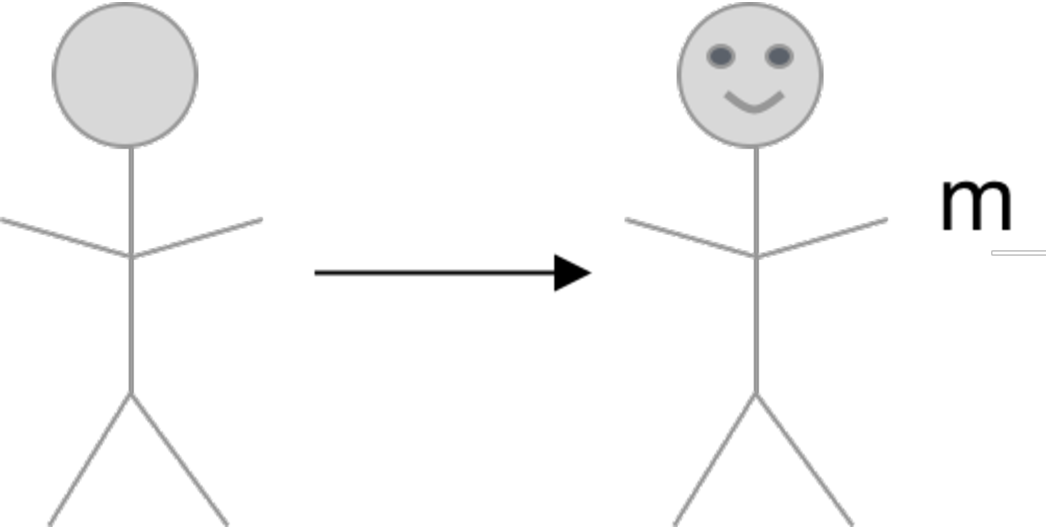
\includegraphics[width=0.5\linewidth]{/home/runner/work/ser2021_mediation_workshop/ser2021_mediation_workshop/img/graphic4a3} 

}

\end{figure}

\hypertarget{is-this-the-estimand-i-want}{%
\subsection{Is this the estimand I want?}\label{is-this-the-estimand-i-want}}

\begin{itemize}
\tightlist
\item
  Makes the most sense if can intervene directly on \(M\)

  \begin{itemize}
  \tightlist
  \item
    and can think of a policy that would set everyone to a single constant
    level \(m \in \mathcal{M}\).
  \item
    J. Pearl calls this \emph{prescriptive}.
  \item
    Can you think of an example?
  \item
    Air pollution, rescue inhaler dosage, hospital visits
  \end{itemize}
\end{itemize}

\emph{What if our research question doesn't involve intervening directly on the
mediator?}

\hypertarget{natural-direct-and-indirect-effects}{%
\section*{Natural direct and indirect effects}\label{natural-direct-and-indirect-effects}}


Natural direct effect (NDE):
\begin{equation*}
  \psi_{\text{NDE}} = \E(Y_{1,M_0}) - \E(Y_{0,M_0})
\end{equation*}

Natural indirect effect (NIE):
\begin{equation*}
  \psi_{\text{NIE}} = \E(Y_{1,M_1}) - \E(Y_{1,M_0})
\end{equation*}

The NDE can also be written as: \(\E_W \sum_m \{\E(Y_{1,m} \mid W) - \E(Y_{0,m} \mid W)\} \P(M_{0}=m \mid W)\)

\begin{itemize}
\tightlist
\item
  Weighted average of controlled direct effects at each level of \(m\).
\item
  If no interaction between \(A\) and \(M\) on \(Y\), then CDE = NDE.
\end{itemize}

\begin{figure}

{\centering 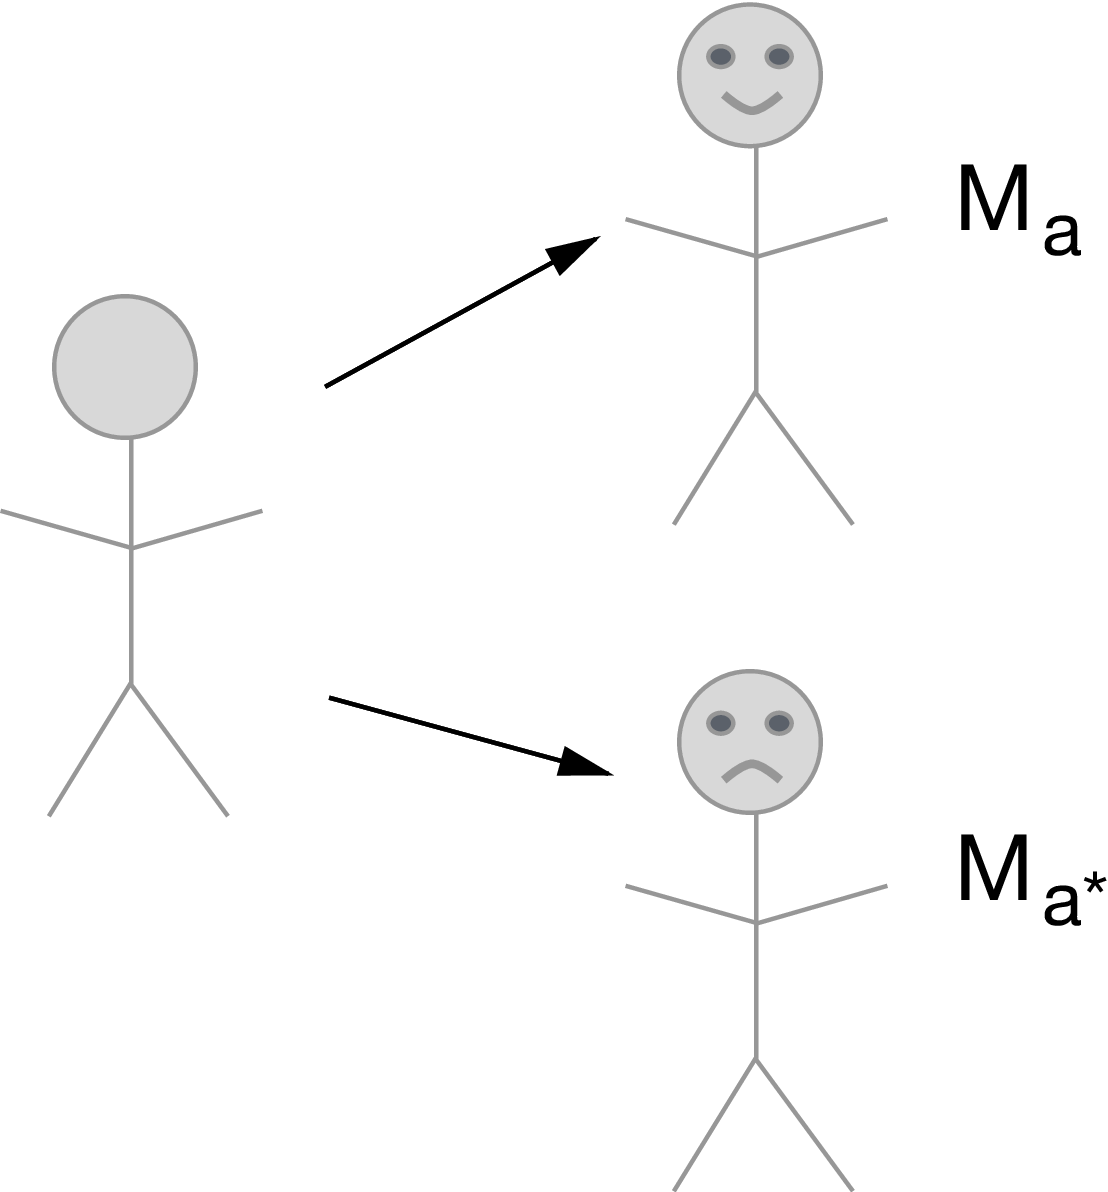
\includegraphics[width=0.5\linewidth]{/home/runner/work/ser2021_mediation_workshop/ser2021_mediation_workshop/img/graphic4a} 

}

\end{figure}

\hypertarget{identification-assumptions}{%
\subsection{Identification assumptions:}\label{identification-assumptions}}

\begin{itemize}
\tightlist
\item
  \(A \indep Y_{a,m} \mid W\)
\item
  \(M \indep Y_{a,m} \mid W, A\)
\item
  \(A \indep M_a \mid W\)
\item
  \(M_{a^{\star}} \indep Y_{a,m} \mid W\)
\item
  and positivity assumptions
\end{itemize}

What does \(M_0 \indep Y_{1,m} \mid W\) mean?

\begin{itemize}
\tightlist
\item
  Conditional on \(W\), knowledge of \(M\) in the absence of treatment \(A\)
  provides no information of the effect of \(A\) on \(Y\).
\item
  Can you think of a data-generating mechanism that would violate this
  assumption?
\item
  Whenever we believe that treatment assignment works through adherence (i.e.,
  almost always), we are violating this assumption.
\end{itemize}

\hypertarget{is-this-the-estimand-i-want-1}{%
\subsection{Is this the estimand I want?}\label{is-this-the-estimand-i-want-1}}

\begin{itemize}
\tightlist
\item
  Makes sense to intervene on \(A\) but not directly on \(M\).
\item
  Want to understand a natural mechanism underlying an association/ total
  effect. J. Pearl calls this \emph{descriptive}.
\item
  NDE + NIE = total effect (ATE).
\item
  Okay with the assumptions.
\end{itemize}

\emph{What if our data structure involves a post-treatment confounder of the
mediator-outcome relationship (e.g., adherence)?}

\begin{figure}

{\centering 
\includegraphics[width=0.2\linewidth]{/home/runner/work/ser2021_mediation_workshop/ser2021_mediation_workshop/img/medDAG2} 

}

\end{figure}

\begin{figure}

{\centering 
\includegraphics[width=0.5\linewidth]{/home/runner/work/ser2021_mediation_workshop/ser2021_mediation_workshop/img/ctndag} 

}

\end{figure}

\hypertarget{interventional-direct-indirect-effects}{%
\section*{Interventional direct/ indirect effects}\label{interventional-direct-indirect-effects}}


\begin{itemize}
\tightlist
\item
  Fully conditional on past
\item
  Conditional SDE: \(\E(Y_{a, g_{M \mid Z, a^{\star}, W}}) - \E(Y_{a^{\star}, g_{M \mid Z, a^{\star}, W}})\)
\item
  Conditional SIE: \(\E(Y_{a, g_{M \mid Z, a, W}}) - \E(Y_{a, g_{M \mid Z, a^{\star}, W}})\)
\item
  Marginal SDE: \(\E(Y_{a, g_{M \mid a^{\star}, W}}) - \E(Y_{a^{\star}, g_{M \mid a^{\star}, W}})\)
\item
  Marginal SIE: \(\E(Y_{a, g_{M \mid a, W}}) - \E(Y_{a, g_{M \mid a^{\star}, W}})\)
\item
  Note that \(g_{M \mid Z, a^{\star}, W}\), \(g_{M \mid a^{\star}, W}\) represents
  stochastic intervention on the mediator, where value \(m\) is drawn with
  probability \(\P(M = m \mid Z, A = a^{\star}, W = w)\),
  \(\P(M = m \mid A = a^{\star}, W = w)\), respectively
\item
  Can you think of an example when you would want the conditional versions?
  Marginal versions?
\end{itemize}

\begin{figure}

{\centering 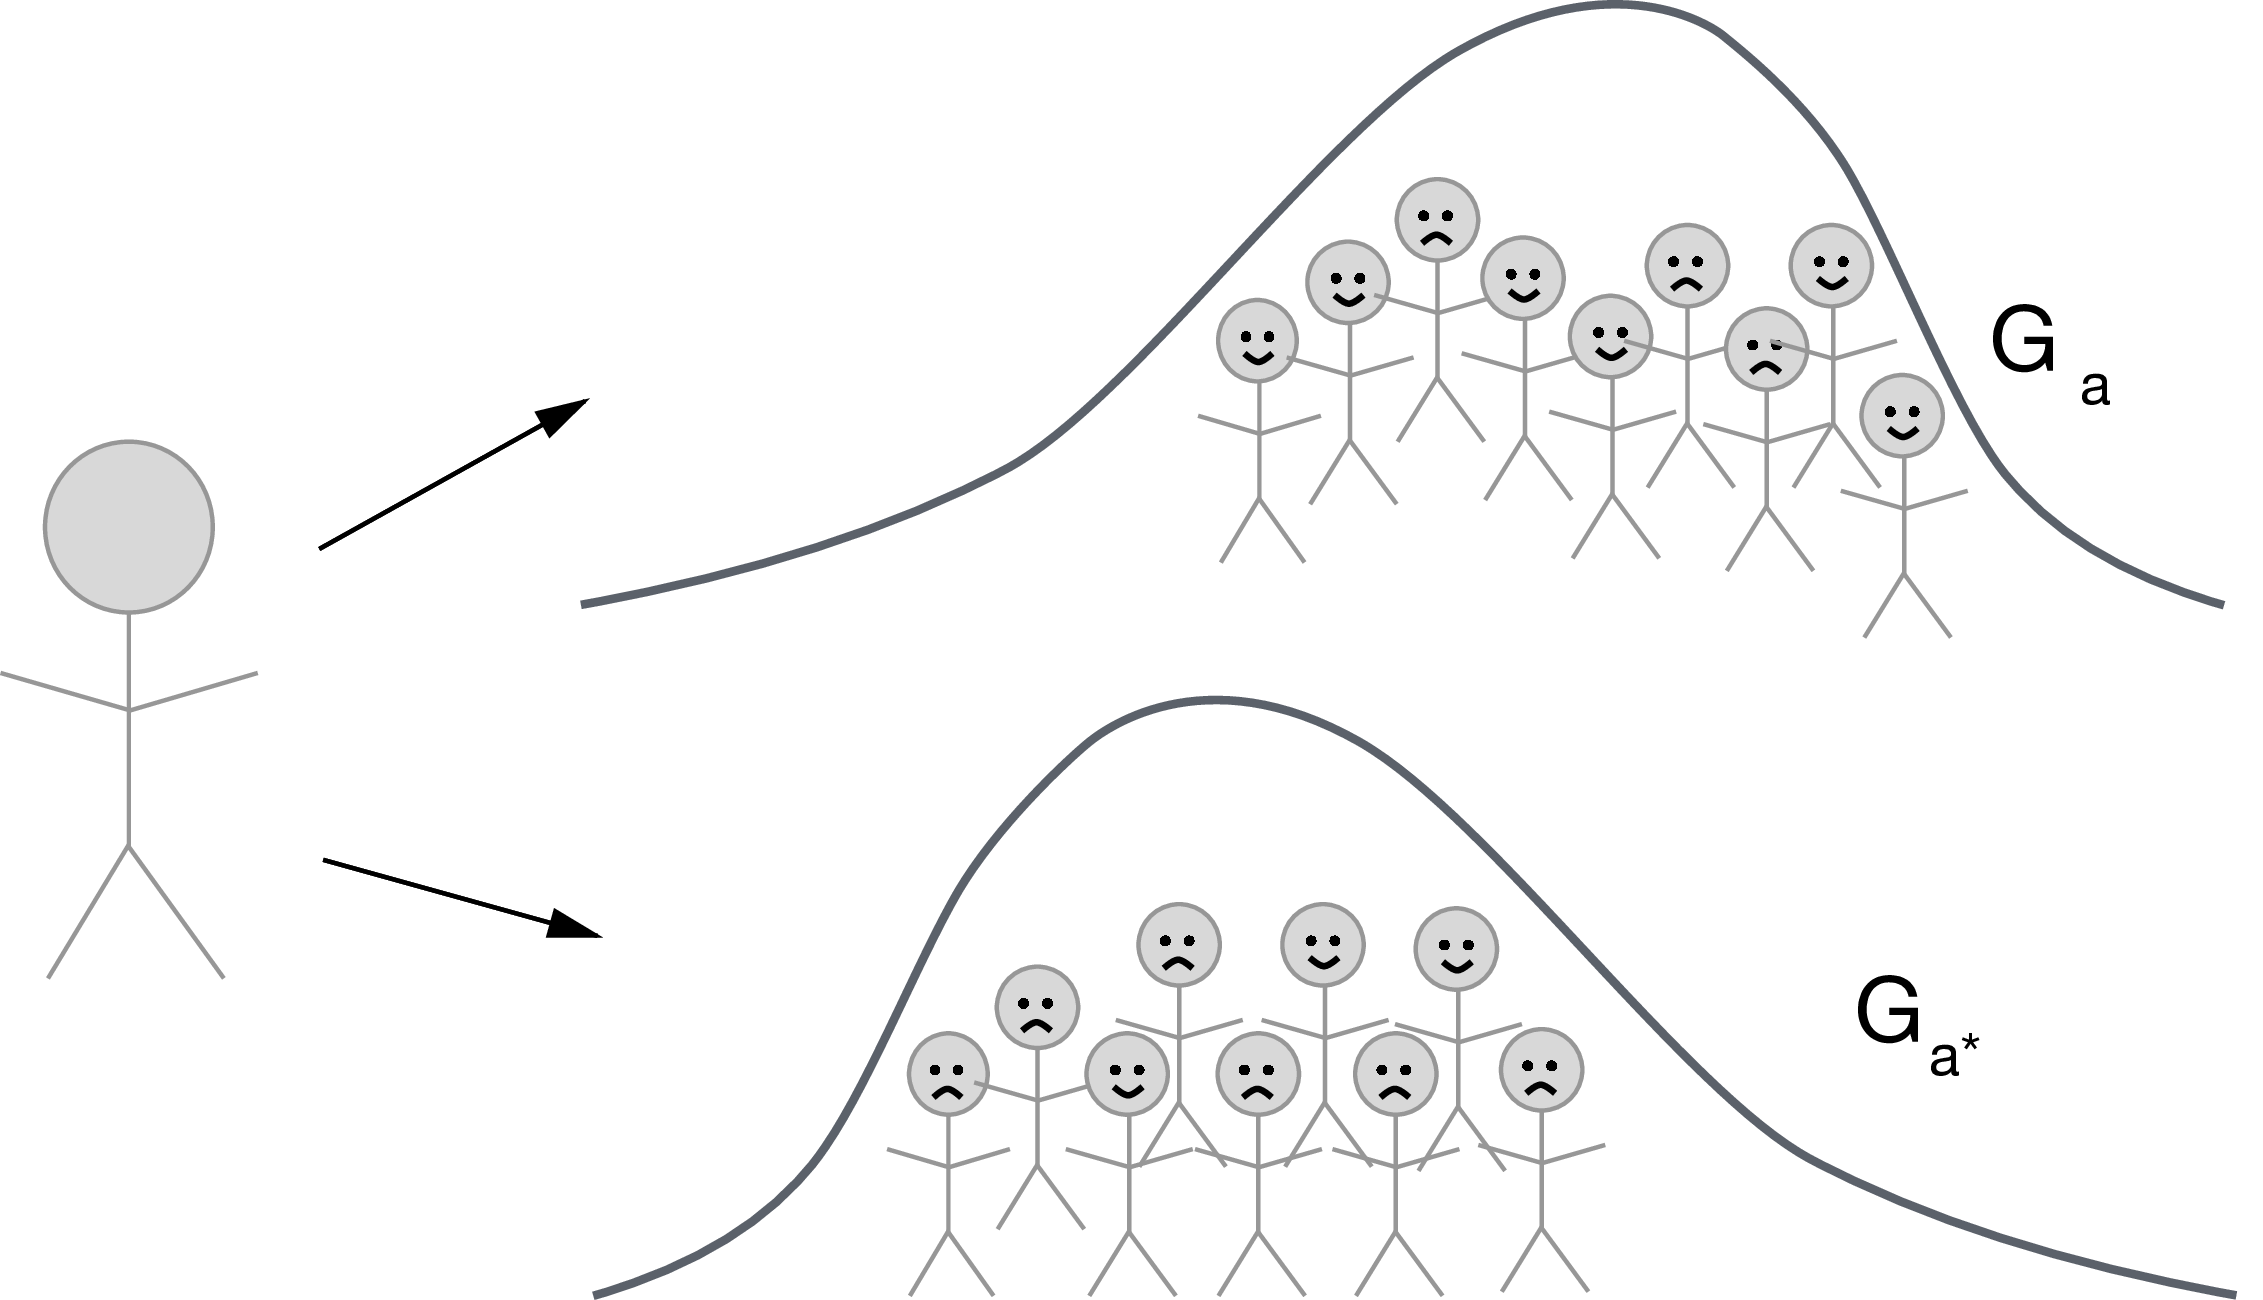
\includegraphics[width=0.5\linewidth]{/home/runner/work/ser2021_mediation_workshop/ser2021_mediation_workshop/img/graphic4b} 

}

\end{figure}

\hypertarget{identification-assumptions-1}{%
\subsection{Identification assumptions:}\label{identification-assumptions-1}}

\begin{itemize}
\tightlist
\item
  \(A \indep Y_{a,m} \mid W\)
\item
  \(M \indep Y_{a,m} \mid W, A\)
\item
  \(A \indep M_a \mid W\)
\item
  and positivity assumptions.
\end{itemize}

Is this the estimand I want?

\begin{itemize}
\tightlist
\item
  Makes sense to intervene on \(A\) but not directly on \(M\).
\item
  Goal is to understand a natural mechanism underlying an association or total
  effect.
\item
  Okay with the assumptions!
\end{itemize}

\hypertarget{estimand-summary}{%
\section*{Estimand Summary}\label{estimand-summary}}


\begin{figure}

{\centering 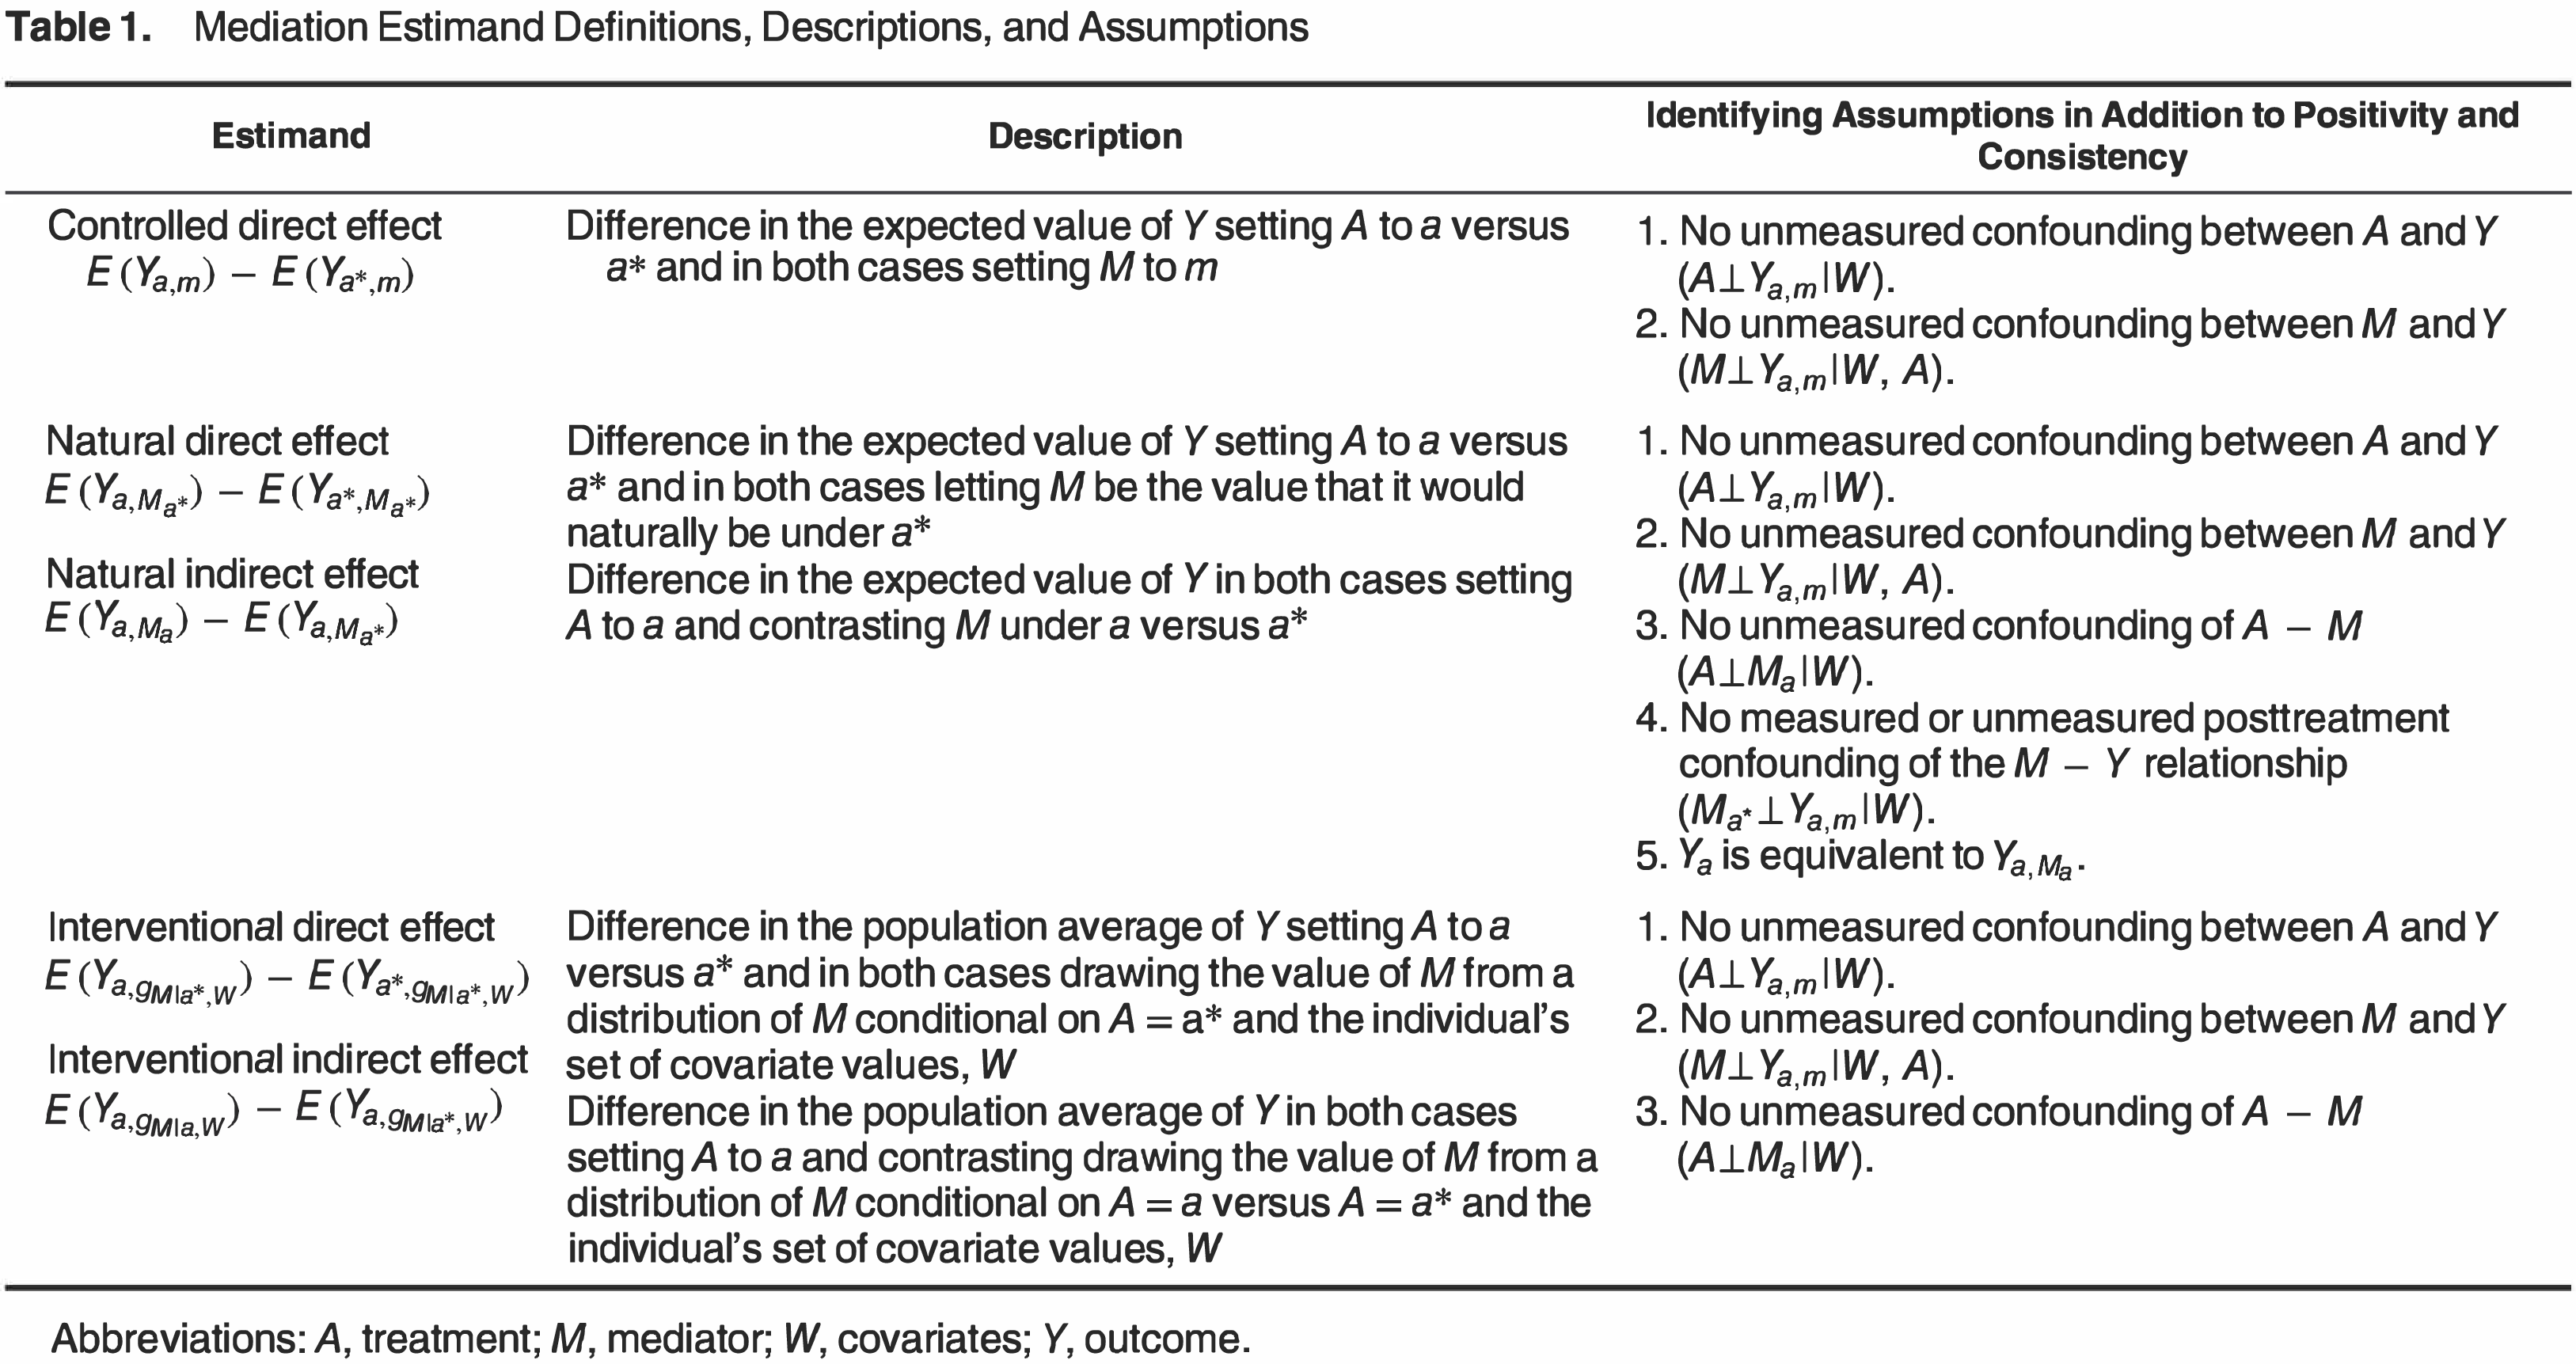
\includegraphics[width=1\linewidth]{/home/runner/work/ser2021_mediation_workshop/ser2021_mediation_workshop/img/table1} 

}

\end{figure}

\hypertarget{estimandirl}{%
\chapter{How to choose an estimand: Real world example}\label{estimandirl}}

\hypertarget{comparative-effectivness-of-two-medications-for-opioid-use-disorder-oud}{%
\section{Comparative effectivness of two medications for opioid use disorder (OUD)}\label{comparative-effectivness-of-two-medications-for-opioid-use-disorder-oud}}

\begin{figure}

{\centering 
\includegraphics[width=0.5\linewidth]{/home/runner/work/ser2021_mediation_workshop/ser2021_mediation_workshop/img/ctndag} 

}

\end{figure}

\emph{Motivation}: Opposite overall treatment effects for homeless versus
nonhomeless participants.

\begin{figure}

{\centering 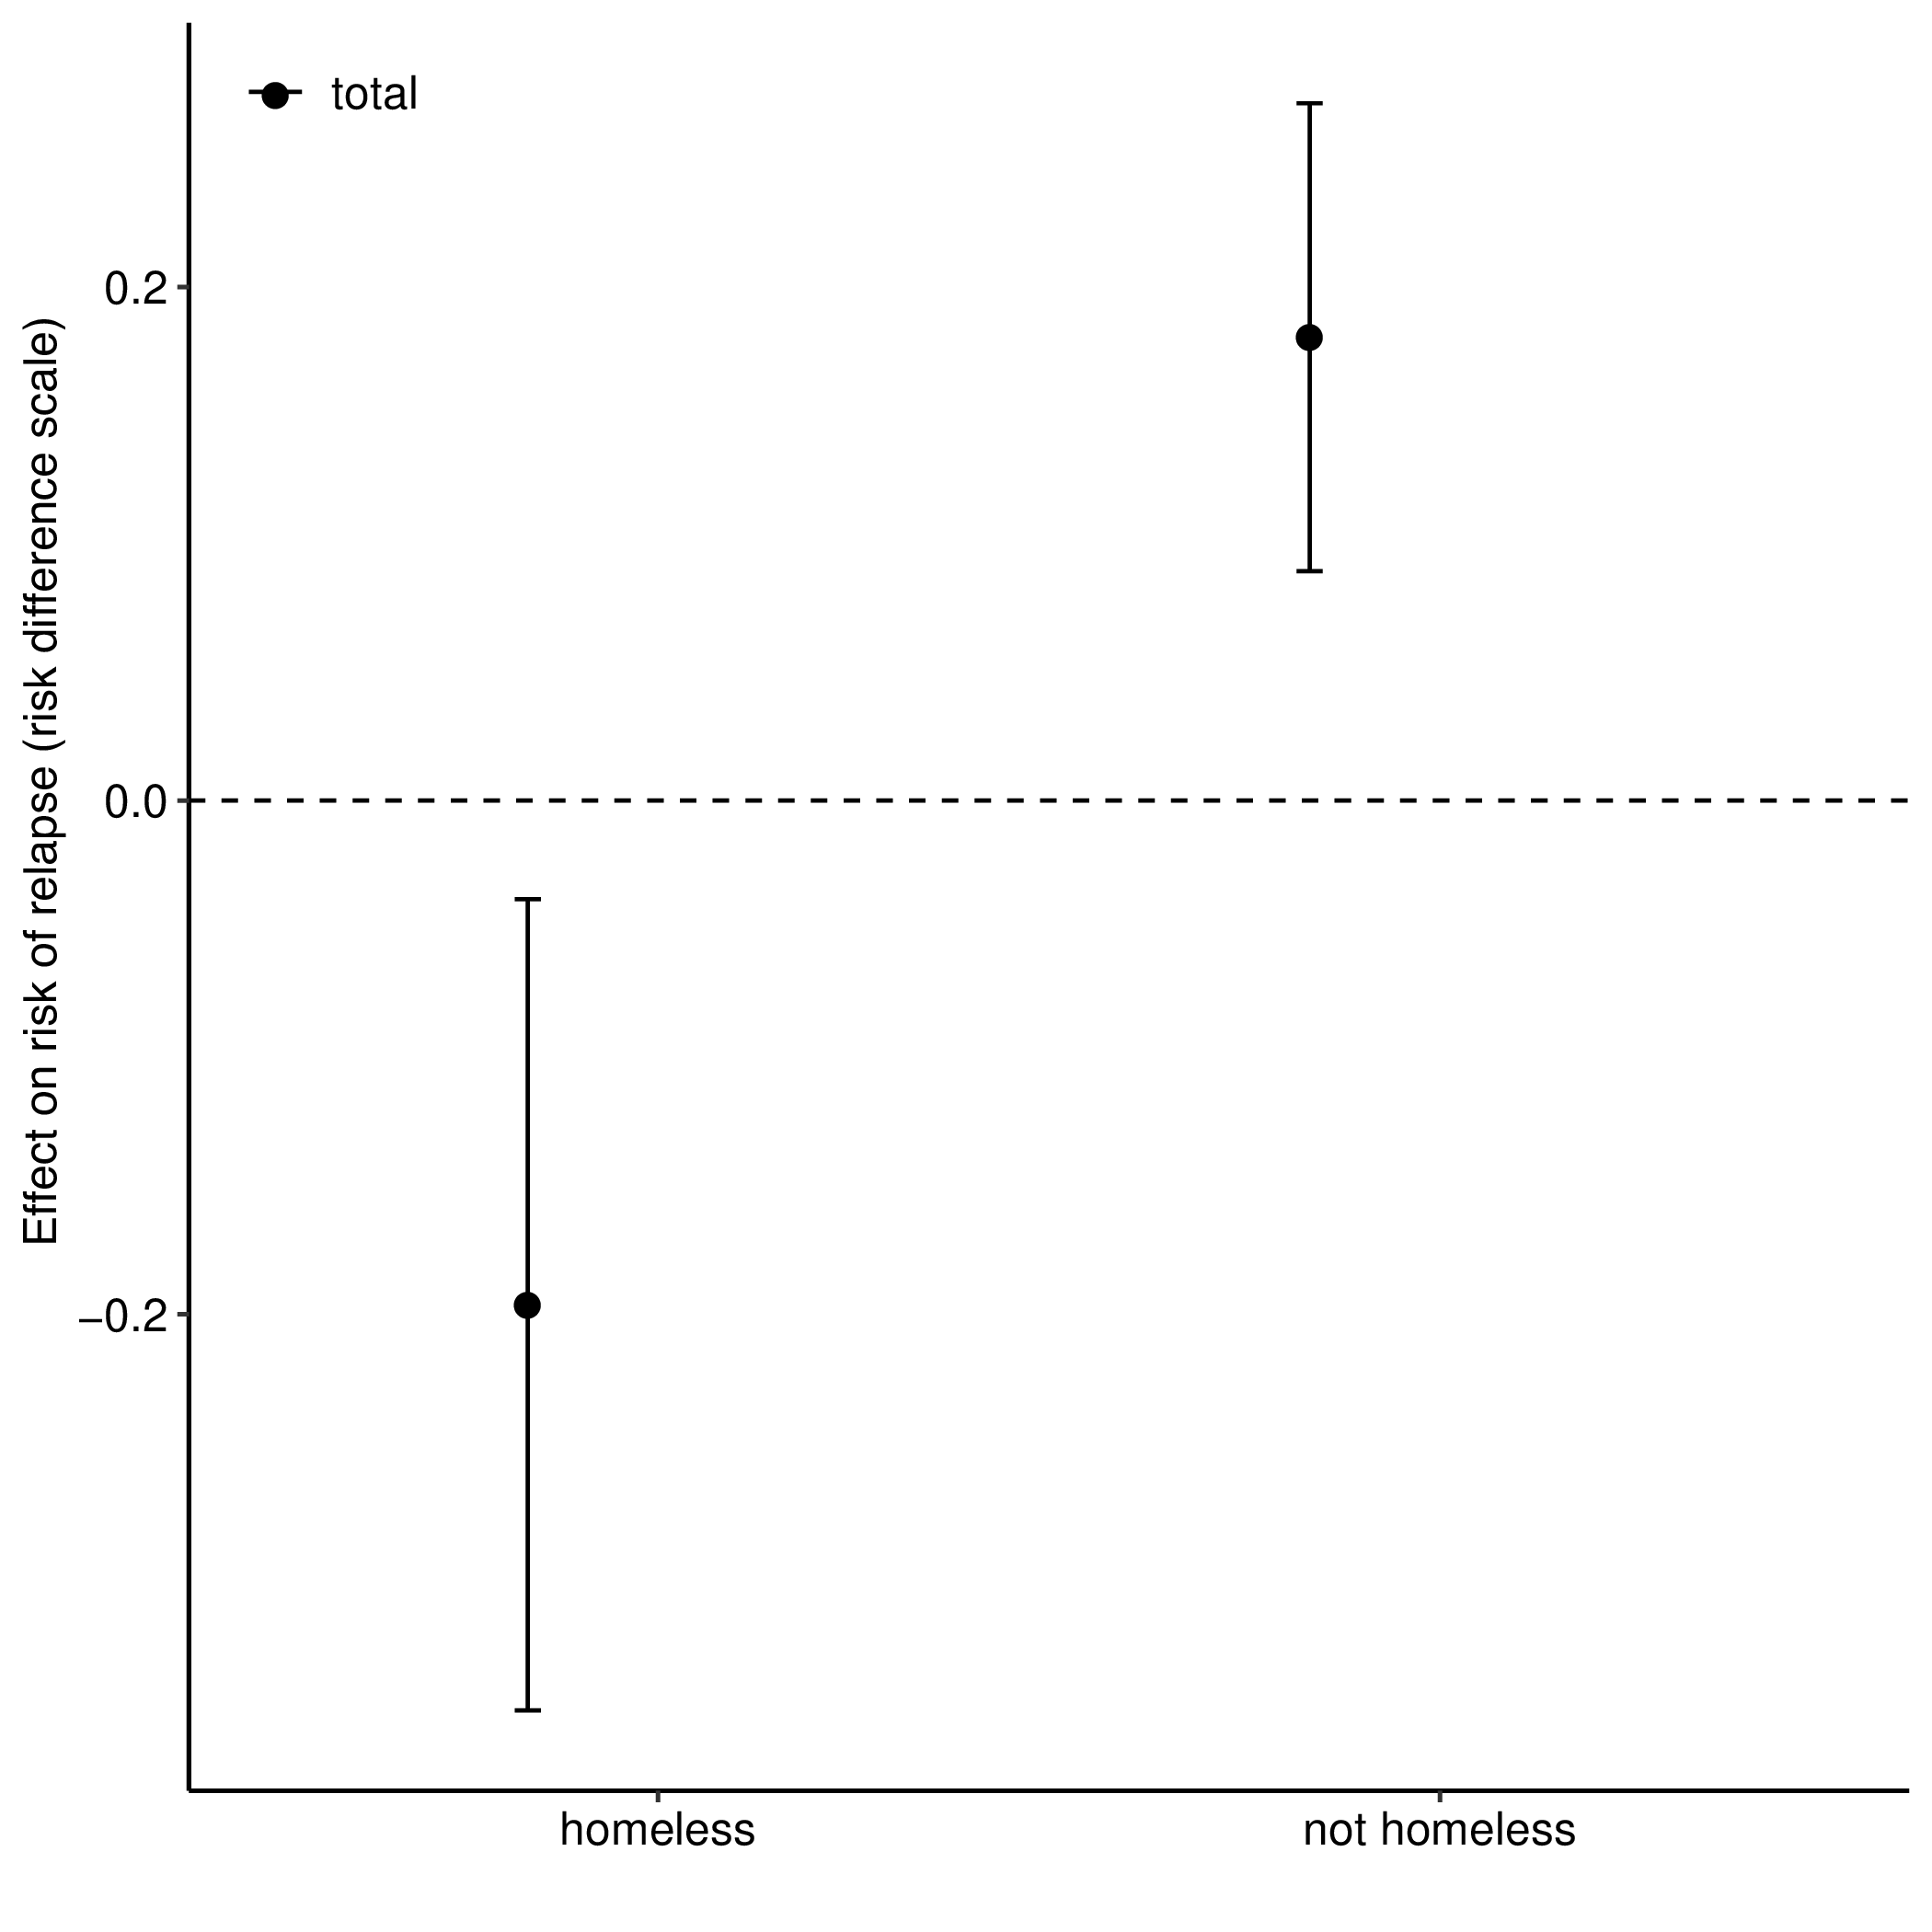
\includegraphics[width=0.5\linewidth]{/home/runner/work/ser2021_mediation_workshop/ser2021_mediation_workshop/img/tmleesttotal} 

}

\end{figure}

\hypertarget{getting-specific-about-the-question}{%
\subsection{Getting specific about the question}\label{getting-specific-about-the-question}}

To what extent does the indirect effect through mediators of adherence, pain,
and depressive symptoms explain the differences in treatment effects on OUD
relapse for homeless and nonhomeless individuals?

What estimand do we want?

\begin{itemize}
\tightlist
\item
  Can we set \(M=m\) (i.e., same value) for everyone?
\item
  Are we interested in estimating indirect effects?
\end{itemize}

\(\rightarrow\) So, \emph{not} controlled direct effect.

\begin{itemize}
\tightlist
\item
  Do we have an intermediate confounder?
\item
  Yes, and it's important.
\end{itemize}

\(\rightarrow\) So, \emph{not} natural (in)direct effects.

\begin{itemize}
\tightlist
\item
  So, we're left with the interventional direct and indirect effects.
\item
  Do we want to estimate the path through treatment initiation (\(Z\))?
\item
  Yes, so, \emph{not} the conditional versions of these effects.
\item
  Estimands:

  \begin{itemize}
  \tightlist
  \item
    Direct effect: \(\E(Y_{1,g_0} - Y_{0,g_0})\)
  \item
    Indirect effect: \(\E(Y_{1,g_1} - Y_{1,g_0})\)
  \end{itemize}
\item
  Need to incorporate multiple and continuous mediators
\end{itemize}

\hypertarget{interventional}{%
\chapter{The Interventional Direct and Indirect Effects}\label{interventional}}

{[}TO FILL IN{]}

\hypertarget{estimation-of-natural-indirect-effects-interventional-indirect-effects}{%
\chapter{Estimation of natural (in)direct effects, interventional (in)direct effects}\label{estimation-of-natural-indirect-effects-interventional-indirect-effects}}

\hypertarget{interventional-direct-and-indirect-effects}{%
\section{Interventional direct and indirect effects}\label{interventional-direct-and-indirect-effects}}

Recall:

\begin{figure}

{\centering 
\includegraphics[width=0.5\linewidth]{/home/runner/work/ser2021_mediation_workshop/ser2021_mediation_workshop/img/medDAG2} 

}

\end{figure}

We define the interventional direct effect as:
\begin{equation*}
  \psi_{\text{PIDE}} = \E(Y_{a^\prime,g_{M \mid a^\star,W}}) -
    \E(Y_{a\star,g_{M \mid a^\star,W}}),
\end{equation*}
and the interventional indirect effect as:
\begin{equation*}
  \psi_{\text{PIIE}} = \E(Y_{a^\prime,g_{M \mid a^\prime,W}}) -
    \E(Y_{a^\prime,g_{M \mid a^\star,W}}).
\end{equation*}

\hypertarget{simple-case-for-intuition}{%
\section{Simple case for intuition}\label{simple-case-for-intuition}}

Consider a simple data structure \(O=(W, A, Z, M, Y)\). This SCM is represented in
the above DAG and the following causal models:
\begin{align*}
  W &= f(U_W)\\
  A &= f(U_A)\\
  Z &= f(A, W, U_Z)\\
  M &= f(Z, A, W, U_M)\\
  Y &= f(M, Z, A, W, U_Y),
\end{align*}
where (\(U_W, U_A, U_Z, U_M, U_Y\)) are exogenous random errors. We assume \(A\) is
a single binary treatment, \(Z\) is a single binary intermediate confounder, \(M\)
is a single binary mediator. There are no restrictions on the distribution of
\(W\) or \(Y\).

\(g_{M \mid a^\prime,W}\) represents a stochastic draw from the counterfactual,
conditional distribution of \(M\), as described by
\citet{vanderweele2016mediation}:
\begin{equation*}
  g_{M \mid A,W}(m, a^{\star}, W) \equiv g_{M \mid a^{\star}, W}(W) =
    \sum_{z=0}^1 \P(M=1 \mid Z=z,W) \P(Z=z \mid A=a^{\star}, W).
\end{equation*}
In what follows, we are going to assume that \(g_{M \mid A,W}(m, a^{\star}, W)\)
is known, estimated from observed data, which we call
\(\hat{g}_{M \mid a^{\star}, W}\). This is going to slightly alter the usual
identification assumptions such that we no longer need to assume exchangeability
of \(A\) and the counterfactual \(M\) values. This means the remaining assumptions
are the same as those for controlled direct effects.

\hypertarget{estimation-using-g-computation}{%
\subsection{Estimation using G-Computation}\label{estimation-using-g-computation}}

The estimand \(E(Y_{a^\prime, \hat{g}_{M \mid a^\star,W}})\) can be identified
via sequential regression, which provides the framework for the
G-computation-based estimator. The procedure is as follows

\begin{enumerate}
\def\labelenumi{\arabic{enumi}.}
\tightlist
\item
  Fit a regression of \(Y\) on \(M,Z,W\). Predict outcome values under under
  \(M=m\). We'll call the result \(\bar{Q}_Y(M,Z,W)\).
\item
  Integrate out \(M\) under our stochastic intervention
  \(\hat{g}_{M \mid a^{\star}, W}\). We can do this by evaluating
  \(\E(Y \mid M=m,Z=z,W)\) at each \(m\) and multiplying it by the probability
  that \(M=m\) under \(\hat{g}_{M \mid a^{\star}, W}\), summing over all \(m\).
  We'll call the results \(\bar{Q}^{g}_M(Z,W)\).
\item
  Integrate out \(Z\) and set \(A=a^\prime\). Again, we can do this by evaluating
  the predicted values from Step 2, setting \(A=a^\prime\), and at each \(z\),
  multiplying the prediction by the probability that \(Z=z\) under \(A=a^\prime\).
  We'll call the result \(\bar{Q}^{a^\prime}_Z(W)\).
\item
  Taking the sample mean (marginalizing over \(W\)) gives the parameter
  estimate.
\end{enumerate}

\hypertarget{estimate-with-doubly-robust-methods-based-on-the-eif}{%
\subsection{Estimate with doubly robust methods based on the EIF}\label{estimate-with-doubly-robust-methods-based-on-the-eif}}

The EIF for the parameter \(\Psi(P)(a^{\prime}, \hat{g}_{M \mid a^{\star},W})\),
where, again, \(\hat{g}_{M \mid a^{\star}, W}\) is assumed known, is given by:
\begin{align*}
  D^{\star}(a^{\prime}, \hat{g}_{M \mid a^{\star}, W}) &= \sum_{k=0}^2
      D_k^{\star}(a^{\prime}, \hat{g}_{M \mid a^{\star}, W}), \text{ where }\\
  D^{\star}_0(a^{\prime}, \hat{g}_{M \mid a^{\star}, W}) &=
      \bar{Q}^{a^{\prime}}_{Z(W)} -
      \Psi(P)(a^{\prime}, \hat{g}_{M \mid a^{\star}, W})\\
  D^{\star}_1(a^{\prime}, \hat{g}_{M \mid a^{\star}, W}) &=
      \frac{I(A=a^{\prime})}{\P(A=a^{\prime} \mid W)}(\bar{Q}^{\hat{g}}_M(Z,W)
      - \bar{Q}^{a^{\prime}}_{Z(W)})\\
  D^{\star}_2(a^{\prime}, \hat{g}_{M \mid a^{\star}, W}) &=
      \frac{I(A=a^{\prime})\{I(M=1) \hat{g}_{M \mid a^{\star}, W} +
      I(M=0)(1-\hat{g}_{M \mid a^{\star}, W}) \}}{\P(A=a^{\prime}}
      &\times (Y-\bar{Q}_{Y(M,Z,W)}).
\end{align*}

\hypertarget{estimate-using-tmle}{%
\subsection{Estimate using TMLE}\label{estimate-using-tmle}}

\begin{enumerate}
\def\labelenumi{\arabic{enumi}.}
\tightlist
\item
  We estimate \(g_{Z \mid a^{\star}, W}(W) = \P(Z=1 \mid A=a^{\star}, W)\) from
  a logistic regression of \(Z\) on \(A, W\) setting \(A=a^{\star}\).
\item
  We then estimate \(g_{M \mid z,W}(W) = \P(M=1 \mid Z=z, W)\) from a logistic
  regression of \(M\) on \(Z, W\), setting \(z=\{0,1\}\).
\item
  We use these quantities to calculate \(\hat{g}_{M \mid a^{\star}, W} = \hat{g}_{M \mid z=1,W}\hat{g}_{Z \mid a^{\star}, W} + \hat{g}_{M \mid z=0,W}(1-\hat{g}_{Z|a^{\star}, W})\).
\end{enumerate}

\begin{Shaded}
\begin{Highlighting}[]
\NormalTok{zmodel <-}\StringTok{ "z ~ a + w1 "}
\NormalTok{mmodel <-}\StringTok{ "m ~ z + w1"}
\NormalTok{ymodel <-}\StringTok{ "y ~ m + z*w1"}

\CommentTok{# make gm and get counterfactual predictions}
\NormalTok{zfit <-}\StringTok{ }\KeywordTok{glm}\NormalTok{(}\DataTypeTok{formula =}\NormalTok{ zmodel, }\DataTypeTok{family =} \StringTok{"binomial"}\NormalTok{, }\DataTypeTok{data =}\NormalTok{ obsdat)}
\NormalTok{mfit <-}\StringTok{ }\KeywordTok{glm}\NormalTok{(}\DataTypeTok{formula =}\NormalTok{ mmodel, }\DataTypeTok{family =} \StringTok{"binomial"}\NormalTok{, }\DataTypeTok{data =}\NormalTok{ obsdat)}

\NormalTok{za0 <-}\StringTok{ }\KeywordTok{predict}\NormalTok{(zfit, }\DataTypeTok{newdata =} \KeywordTok{data.frame}\NormalTok{(}\DataTypeTok{w1 =}\NormalTok{ obsdat}\OperatorTok{$}\NormalTok{w1, }\DataTypeTok{a =} \DecValTok{0}\NormalTok{),}
               \DataTypeTok{type =} \StringTok{"response"}\NormalTok{)}
\NormalTok{za1 <-}\StringTok{ }\KeywordTok{predict}\NormalTok{(zfit, }\DataTypeTok{newdata =} \KeywordTok{data.frame}\NormalTok{(}\DataTypeTok{w1 =}\NormalTok{ obsdat}\OperatorTok{$}\NormalTok{w1, }\DataTypeTok{a =} \DecValTok{1}\NormalTok{),}
               \DataTypeTok{type =} \StringTok{"response"}\NormalTok{)}

\NormalTok{mz1 <-}\StringTok{ }\KeywordTok{predict}\NormalTok{(mfit, }\DataTypeTok{newdata =} \KeywordTok{data.frame}\NormalTok{(}\DataTypeTok{w1 =}\NormalTok{ obsdat}\OperatorTok{$}\NormalTok{w1, }\DataTypeTok{z =} \DecValTok{1}\NormalTok{),}
               \DataTypeTok{type =} \StringTok{"response"}\NormalTok{)}
\NormalTok{mz0 }\OperatorTok{<}\StringTok{ }\OperatorTok{-}\KeywordTok{predict}\NormalTok{(mfit, }\DataTypeTok{newdata =} \KeywordTok{data.frame}\NormalTok{(}\DataTypeTok{w1 =}\NormalTok{ obsdat}\OperatorTok{$}\NormalTok{w1, }\DataTypeTok{z =} \DecValTok{0}\NormalTok{),}
               \DataTypeTok{type =} \StringTok{"response"}\NormalTok{)}

\NormalTok{gm0 <-}\StringTok{ }\NormalTok{(mz1 }\OperatorTok{*}\StringTok{ }\NormalTok{za0) }\OperatorTok{+}\StringTok{ }\NormalTok{(mz0 }\OperatorTok{*}\StringTok{ }\NormalTok{(}\DecValTok{1} \OperatorTok{-}\StringTok{ }\NormalTok{za0))}
\NormalTok{gma1 <-}\StringTok{ }\NormalTok{(mz1 }\OperatorTok{*}\StringTok{ }\NormalTok{za1) }\OperatorTok{+}\StringTok{ }\NormalTok{(mz0 }\OperatorTok{*}\StringTok{ }\NormalTok{(}\DecValTok{1} \OperatorTok{-}\StringTok{ }\NormalTok{za1))}
\end{Highlighting}
\end{Shaded}

\begin{enumerate}
\def\labelenumi{\arabic{enumi}.}
\setcounter{enumi}{3}
\tightlist
\item
  To obtain an estimate of \(\bar{Q}_{Y}(M,Z,W)\), predict values of \(Y\) from a
  regression of \(Y\) on \(M,Z,W\), setting \(m=1\) and \(m=0\), giving
  \(\hat{Y}(m=1, z, w)\) and \(\hat{Y}(m=0, z, w)\).
\end{enumerate}

\begin{Shaded}
\begin{Highlighting}[]
\NormalTok{tmpdat}\OperatorTok{$}\NormalTok{qyinit <-}\StringTok{ }\KeywordTok{cbind}\NormalTok{(}
  \KeywordTok{predict}\NormalTok{(}\KeywordTok{glm}\NormalTok{(}\DataTypeTok{formula =}\NormalTok{ ymodel, }\DataTypeTok{family =} \StringTok{"binomial"}\NormalTok{,}
              \DataTypeTok{data =} \KeywordTok{data.frame}\NormalTok{(}\KeywordTok{cbind}\NormalTok{(datw, }\DataTypeTok{z =}\NormalTok{ z, }\DataTypeTok{m =}\NormalTok{ m, }\DataTypeTok{y =}\NormalTok{ y))),}
          \DataTypeTok{newdata =} \KeywordTok{data.frame}\NormalTok{(}\KeywordTok{cbind}\NormalTok{(datw, }\DataTypeTok{z =}\NormalTok{ z, }\DataTypeTok{m =}\NormalTok{ m)), }\DataTypeTok{type =} \StringTok{"response"}\NormalTok{),}
  \KeywordTok{predict}\NormalTok{(}\KeywordTok{glm}\NormalTok{(}\DataTypeTok{formula =}\NormalTok{ ymodel, }\DataTypeTok{family =} \StringTok{"binomial"}\NormalTok{,}
              \DataTypeTok{data =} \KeywordTok{data.frame}\NormalTok{(}\KeywordTok{cbind}\NormalTok{(datw, }\DataTypeTok{z =}\NormalTok{ z, }\DataTypeTok{m =}\NormalTok{ m, }\DataTypeTok{y =}\NormalTok{ y))),}
          \DataTypeTok{newdata =} \KeywordTok{data.frame}\NormalTok{(}\KeywordTok{cbind}\NormalTok{(datw, }\DataTypeTok{z =}\NormalTok{ z, }\DataTypeTok{m =} \DecValTok{0}\NormalTok{)), }\DataTypeTok{type =} \StringTok{"response"}\NormalTok{),}
  \KeywordTok{predict}\NormalTok{(}\KeywordTok{glm}\NormalTok{(}\DataTypeTok{formula =}\NormalTok{ ymodel, }\DataTypeTok{family =} \StringTok{"binomial"}\NormalTok{,}
              \DataTypeTok{data =} \KeywordTok{data.frame}\NormalTok{(}\KeywordTok{cbind}\NormalTok{(datw, }\DataTypeTok{z =}\NormalTok{ z, }\DataTypeTok{m =}\NormalTok{ m, }\DataTypeTok{y =}\NormalTok{ y))),}
          \DataTypeTok{newdata =} \KeywordTok{data.frame}\NormalTok{(}\KeywordTok{cbind}\NormalTok{(datw, }\DataTypeTok{z =}\NormalTok{ z, }\DataTypeTok{m =} \DecValTok{1}\NormalTok{)), }\DataTypeTok{type =} \StringTok{"response"}\NormalTok{)}
\NormalTok{)}
\end{Highlighting}
\end{Shaded}

\begin{enumerate}
\def\labelenumi{\arabic{enumi}.}
\setcounter{enumi}{4}
\tightlist
\item
  Estimate the weights to be used for the initial targeting step:
  \begin{equation*}
     h_1(a) = \frac{I(A=a)\{I(M=1)\hat{g}_{M \mid a^{\star}, W} +
       I(M=0)(1-\hat{g}_{M \mid a^{\star}, W}) \}}{\P(A=a)\{I(M=1)
       g_{M \mid Z,W} + I(M=0)(1-g_{M \mid Z,W}) \}}
  \end{equation*}
\end{enumerate}

\begin{Shaded}
\begin{Highlighting}[]
\NormalTok{psa1 <-}\StringTok{ }\KeywordTok{I}\NormalTok{(a }\OperatorTok{==}\StringTok{ }\DecValTok{1}\NormalTok{) }\OperatorTok{/}\StringTok{ }\KeywordTok{mean}\NormalTok{(a)}
\NormalTok{psa0 <-}\StringTok{ }\KeywordTok{I}\NormalTok{(a }\OperatorTok{==}\StringTok{ }\DecValTok{0}\NormalTok{) }\OperatorTok{/}\StringTok{ }\KeywordTok{mean}\NormalTok{(}\DecValTok{1} \OperatorTok{-}\StringTok{ }\NormalTok{a)}
\NormalTok{mz <-}\StringTok{ }\KeywordTok{predict}\NormalTok{(}\KeywordTok{glm}\NormalTok{(}\DataTypeTok{formula =}\NormalTok{ mmodel, }\DataTypeTok{family =} \StringTok{"binomial"}\NormalTok{,}
                  \DataTypeTok{data =} \KeywordTok{data.frame}\NormalTok{(}\KeywordTok{cbind}\NormalTok{(datw, }\DataTypeTok{z =}\NormalTok{ z, }\DataTypeTok{m =}\NormalTok{ m))),}
              \DataTypeTok{newdata =} \KeywordTok{data.frame}\NormalTok{(}\KeywordTok{cbind}\NormalTok{(datw, }\DataTypeTok{z =}\NormalTok{ z)), }\DataTypeTok{type =} \StringTok{"response"}\NormalTok{)}
\NormalTok{psm <-}\StringTok{ }\NormalTok{(mz }\OperatorTok{*}\StringTok{ }\NormalTok{m) }\OperatorTok{+}\StringTok{ }\NormalTok{((}\DecValTok{1} \OperatorTok{-}\StringTok{ }\NormalTok{mz) }\OperatorTok{*}\StringTok{ }\NormalTok{(}\DecValTok{1} \OperatorTok{-}\StringTok{ }\NormalTok{m))}

\NormalTok{tmpdat}\OperatorTok{$}\NormalTok{ha1gma1 <-}\StringTok{ }\NormalTok{((m }\OperatorTok{*}\StringTok{ }\NormalTok{gma1 }\OperatorTok{+}\StringTok{ }\NormalTok{(}\DecValTok{1} \OperatorTok{-}\StringTok{ }\NormalTok{m) }\OperatorTok{*}\StringTok{ }\NormalTok{(}\DecValTok{1} \OperatorTok{-}\StringTok{ }\NormalTok{gma1)) }\OperatorTok{/}\StringTok{ }\NormalTok{psm) }\OperatorTok{*}\StringTok{ }\NormalTok{psa1 }\OperatorTok{*}\StringTok{ }\NormalTok{svywt}
\NormalTok{tmpdat}\OperatorTok{$}\NormalTok{ha1gma0 <-}\StringTok{ }\NormalTok{((m }\OperatorTok{*}\StringTok{ }\NormalTok{gm }\OperatorTok{+}\StringTok{ }\NormalTok{(}\DecValTok{1} \OperatorTok{-}\StringTok{ }\NormalTok{m) }\OperatorTok{*}\StringTok{ }\NormalTok{(}\DecValTok{1} \OperatorTok{-}\StringTok{ }\NormalTok{gm)) }\OperatorTok{/}\StringTok{ }\NormalTok{psm) }\OperatorTok{*}\StringTok{ }\NormalTok{psa1 }\OperatorTok{*}\StringTok{ }\NormalTok{svywt}
\NormalTok{tmpdat}\OperatorTok{$}\NormalTok{ha0gma0 <-}\StringTok{ }\NormalTok{((m }\OperatorTok{*}\StringTok{ }\NormalTok{gm }\OperatorTok{+}\StringTok{ }\NormalTok{(}\DecValTok{1} \OperatorTok{-}\StringTok{ }\NormalTok{m) }\OperatorTok{*}\StringTok{ }\NormalTok{(}\DecValTok{1} \OperatorTok{-}\StringTok{ }\NormalTok{gm)) }\OperatorTok{/}\StringTok{ }\NormalTok{psm) }\OperatorTok{*}\StringTok{ }\NormalTok{psa0 }\OperatorTok{*}\StringTok{ }\NormalTok{svywt}
\end{Highlighting}
\end{Shaded}

\begin{enumerate}
\def\labelenumi{\arabic{enumi}.}
\setcounter{enumi}{5}
\item
  Estimate \(\hat{\epsilon}\) by setting \(\epsilon\) as the intercept of a
  weighted logistic regression model of \(Y\) with
  \(\text{logit}(\hat{\bar{Q}}_{Y}(M,Z,W))\) as an offset and weights
  \(\hat{h}_{1}(a)\). (Note that this is just one possible TMLE.)
\item
  The estimate of \(\bar{Q}_{Y}(M,Z,W)\) is updated by
  \(\hat{\bar{Q}}^{\star}_{Y}(M,Z,W) = \hat{\bar{Q}}_{Y}(\epsilon_n)(M,Z,W)\).
\end{enumerate}

\begin{Shaded}
\begin{Highlighting}[]
\CommentTok{# for E(Y_\{1,gmastar\})}
\NormalTok{epsilonma1g0 <-}\StringTok{ }\KeywordTok{coef}\NormalTok{(}\KeywordTok{glm}\NormalTok{(y }\OperatorTok{~}\StringTok{ }\DecValTok{1}\NormalTok{, }\DataTypeTok{weights =}\NormalTok{ tmpdat}\OperatorTok{$}\NormalTok{ha1gma0,}
                         \DataTypeTok{offset =}\NormalTok{ (}\KeywordTok{qlogis}\NormalTok{(qyinit[, }\DecValTok{1}\NormalTok{])),}
                         \DataTypeTok{family =} \StringTok{"quasibinomial"}\NormalTok{, }\DataTypeTok{data =}\NormalTok{ tmpdat))}
\NormalTok{tmpdat}\OperatorTok{$}\NormalTok{qyupm0a1g0 <-}\StringTok{ }\KeywordTok{plogis}\NormalTok{(}\KeywordTok{qlogis}\NormalTok{(tmpdat}\OperatorTok{$}\NormalTok{qyinit[, }\DecValTok{2}\NormalTok{]) }\OperatorTok{+}\StringTok{ }\NormalTok{epsilonma1g0)}
\NormalTok{tmpdat}\OperatorTok{$}\NormalTok{qyupm1a1g0 <-}\StringTok{ }\KeywordTok{plogis}\NormalTok{(}\KeywordTok{qlogis}\NormalTok{(tmpdat}\OperatorTok{$}\NormalTok{qyinit[, }\DecValTok{3}\NormalTok{]) }\OperatorTok{+}\StringTok{ }\NormalTok{epsilonma1g0)}

\CommentTok{# for E(Y_\{1,gma\})}
\NormalTok{epsilonma1g1 <-}\StringTok{ }\KeywordTok{coef}\NormalTok{(}\KeywordTok{glm}\NormalTok{(y }\OperatorTok{~}\StringTok{ }\DecValTok{1}\NormalTok{, }\DataTypeTok{weights =}\NormalTok{ tmpdat}\OperatorTok{$}\NormalTok{ha1gma1,}
                         \DataTypeTok{offset =}\NormalTok{ (}\KeywordTok{qlogis}\NormalTok{(qyinit[, }\DecValTok{1}\NormalTok{])),}
                         \DataTypeTok{family =} \StringTok{"quasibinomial"}\NormalTok{, }\DataTypeTok{data =}\NormalTok{ tmpdat))}
\NormalTok{tmpdat}\OperatorTok{$}\NormalTok{qyupm0a1g1 <-}\StringTok{ }\KeywordTok{plogis}\NormalTok{(}\KeywordTok{qlogis}\NormalTok{(tmpdat}\OperatorTok{$}\NormalTok{qyinit[, }\DecValTok{2}\NormalTok{]) }\OperatorTok{+}\StringTok{ }\NormalTok{epsilonma1g1)}
\NormalTok{tmpdat}\OperatorTok{$}\NormalTok{qyupm1a1g1 <-}\StringTok{ }\KeywordTok{plogis}\NormalTok{(}\KeywordTok{qlogis}\NormalTok{(tmpdat}\OperatorTok{$}\NormalTok{qyinit[, }\DecValTok{3}\NormalTok{]) }\OperatorTok{+}\StringTok{ }\NormalTok{epsilonma1g1)}

\CommentTok{# for E(Y_\{0,gmastar\})}
\NormalTok{epsilonma0g0 <-}\StringTok{ }\KeywordTok{coef}\NormalTok{(}\KeywordTok{glm}\NormalTok{(y }\OperatorTok{~}\StringTok{ }\DecValTok{1}\NormalTok{, }\DataTypeTok{weights =}\NormalTok{ tmpdat}\OperatorTok{$}\NormalTok{ha0gma0,}
                         \DataTypeTok{offset =}\NormalTok{ (}\KeywordTok{qlogis}\NormalTok{(qyinit[, }\DecValTok{1}\NormalTok{])),}
                         \DataTypeTok{family =} \StringTok{"quasibinomial"}\NormalTok{, }\DataTypeTok{data =}\NormalTok{ tmpdat))}
\NormalTok{tmpdat}\OperatorTok{$}\NormalTok{qyupm0a0g0 <-}\StringTok{ }\KeywordTok{plogis}\NormalTok{(}\KeywordTok{qlogis}\NormalTok{(tmpdat}\OperatorTok{$}\NormalTok{qyinit[, }\DecValTok{2}\NormalTok{]) }\OperatorTok{+}\StringTok{ }\NormalTok{epsilonma0g0)}
\NormalTok{tmpdat}\OperatorTok{$}\NormalTok{qyupm1a0g0 <-}\StringTok{ }\KeywordTok{plogis}\NormalTok{(}\KeywordTok{qlogis}\NormalTok{(tmpdat}\OperatorTok{$}\NormalTok{qyinit[, }\DecValTok{3}\NormalTok{]) }\OperatorTok{+}\StringTok{ }\NormalTok{epsilonma0g0)}
\end{Highlighting}
\end{Shaded}

\begin{enumerate}
\def\labelenumi{\arabic{enumi}.}
\setcounter{enumi}{7}
\tightlist
\item
  We next integrate out \(M\) from \(\bar{Q}^{\star}_{Y}(M,Z,W)\). First, we
  estimate \(\bar{Q}^{\star}_{Y,n}(M,Z,W)\) setting \(m=1\) and \(m=0\), giving
  \(\bar{Q}^{\star}_Y(m=1, z, w)\) and \(\bar{Q}^{\star}_Y(m=0, z, w)\). Then,
  multiply these predicted values by their probabilities under
  \(\hat{g}_{M \mid a^{\star},W}(W)\) (for \(a \in \{a, a^{\star}\}\)), and add
  them together (i.e., \(\bar{Q}^{\hat{g}}_{M,n}(Z,W) = \hat{Q}^{\star}_Y(m=1, z, w) \hat{g}_{M|a^{\star},W} + \hat{Q}^{\star}_Y(m=0, z, w)(1-\hat{g}_{M|a^{\star},W})\)).
\end{enumerate}

\begin{Shaded}
\begin{Highlighting}[]
\NormalTok{tmpdat}\OperatorTok{$}\NormalTok{Qma1g0 <-}\StringTok{ }\NormalTok{tmpdat}\OperatorTok{$}\NormalTok{qyupm0a1g0 }\OperatorTok{*}\StringTok{ }\NormalTok{(}\DecValTok{1} \OperatorTok{-}\StringTok{ }\NormalTok{gm) }\OperatorTok{+}\StringTok{ }\NormalTok{tmpdat}\OperatorTok{$}\NormalTok{qyupm1a1g0 }\OperatorTok{*}\StringTok{ }\NormalTok{gm}
\NormalTok{tmpdat}\OperatorTok{$}\NormalTok{Qma1g1 <-}\StringTok{ }\NormalTok{tmpdat}\OperatorTok{$}\NormalTok{qyupm0a1g1 }\OperatorTok{*}\StringTok{ }\NormalTok{(}\DecValTok{1} \OperatorTok{-}\StringTok{ }\NormalTok{gma1) }\OperatorTok{+}\StringTok{ }\NormalTok{tmpdat}\OperatorTok{$}\NormalTok{qyupm1a1g1 }\OperatorTok{*}\StringTok{ }\NormalTok{gma1}
\NormalTok{tmpdat}\OperatorTok{$}\NormalTok{Qma0g0 <-}\StringTok{ }\NormalTok{tmpdat}\OperatorTok{$}\NormalTok{qyupm0a0g0 }\OperatorTok{*}\StringTok{ }\NormalTok{(}\DecValTok{1} \OperatorTok{-}\StringTok{ }\NormalTok{gm) }\OperatorTok{+}\StringTok{ }\NormalTok{tmpdat}\OperatorTok{$}\NormalTok{qyupm1a0g0 }\OperatorTok{*}\StringTok{ }\NormalTok{gm}
\end{Highlighting}
\end{Shaded}

\begin{enumerate}
\def\labelenumi{\arabic{enumi}.}
\setcounter{enumi}{8}
\tightlist
\item
  We now fit a regression of \(\bar{Q}^{\hat{g},\star}_{M,n}(Z,W)\) on \(W\)
  among those with \(A=a^\prime\). We call the predicted values from this
  regression \(\hat{\bar{Q}}^{a^\prime}_{Z}(W)\).
\end{enumerate}

\begin{Shaded}
\begin{Highlighting}[]
\NormalTok{Qzfita1g0 <-}\StringTok{ }\KeywordTok{glm}\NormalTok{(}\DataTypeTok{formula =} \KeywordTok{paste}\NormalTok{(}\StringTok{"Qma1g0"}\NormalTok{, qmodel, }\DataTypeTok{sep =} \StringTok{"~"}\NormalTok{),}
                 \DataTypeTok{data =}\NormalTok{ tmpdat[tmpdat}\OperatorTok{$}\NormalTok{a }\OperatorTok{==}\StringTok{ }\DecValTok{1}\NormalTok{, ], }\DataTypeTok{family =} \StringTok{"quasibinomial"}\NormalTok{)}
\NormalTok{Qzfita1g1 <-}\StringTok{ }\KeywordTok{glm}\NormalTok{(}\DataTypeTok{formula =} \KeywordTok{paste}\NormalTok{(}\StringTok{"Qma1g1"}\NormalTok{, qmodel, }\DataTypeTok{sep =} \StringTok{"~"}\NormalTok{),}
                 \DataTypeTok{data =}\NormalTok{ tmpdat[tmpdat}\OperatorTok{$}\NormalTok{a }\OperatorTok{==}\StringTok{ }\DecValTok{1}\NormalTok{, ], }\DataTypeTok{family =} \StringTok{"quasibinomial"}\NormalTok{)}
\NormalTok{Qzfita0g0 <-}\StringTok{ }\KeywordTok{glm}\NormalTok{(}\DataTypeTok{formula =} \KeywordTok{paste}\NormalTok{(}\StringTok{"Qma0g0"}\NormalTok{, qmodel, }\DataTypeTok{sep =} \StringTok{"~"}\NormalTok{),}
                 \DataTypeTok{data =}\NormalTok{ tmpdat[tmpdat}\OperatorTok{$}\NormalTok{a }\OperatorTok{==}\StringTok{ }\DecValTok{0}\NormalTok{, ], }\DataTypeTok{family =} \StringTok{"quasibinomial"}\NormalTok{)}

\NormalTok{Qza1g0 <-}\StringTok{ }\KeywordTok{predict}\NormalTok{(Qzfita1g0, }\DataTypeTok{type =} \StringTok{"response"}\NormalTok{, }\DataTypeTok{newdata =}\NormalTok{ tmpdat)}
\NormalTok{Qza1g1 <-}\StringTok{ }\KeywordTok{predict}\NormalTok{(Qzfita1g1, }\DataTypeTok{type =} \StringTok{"response"}\NormalTok{, }\DataTypeTok{newdata =}\NormalTok{ tmpdat)}
\NormalTok{Qza0g0 <-}\StringTok{ }\KeywordTok{predict}\NormalTok{(Qzfita0g0, }\DataTypeTok{type =} \StringTok{"response"}\NormalTok{, }\DataTypeTok{newdata =}\NormalTok{ tmpdat)}
\end{Highlighting}
\end{Shaded}

(Note that if \(A\) were not randomly assigned, we would need to complete a
second targeting step.)

\begin{enumerate}
\def\labelenumi{\arabic{enumi}.}
\setcounter{enumi}{9}
\tightlist
\item
  The empirical mean of these predicted values is the TML estimate of
  \(\Psi(P)(a^\prime, \hat{g}_{M \mid a^{\star}, W})\).
\end{enumerate}

\begin{Shaded}
\begin{Highlighting}[]
\NormalTok{tmlea1m0 <-}\StringTok{ }\KeywordTok{sum}\NormalTok{(Qzupa1g0 }\OperatorTok{*}\StringTok{ }\NormalTok{svywt) }\OperatorTok{/}\StringTok{ }\KeywordTok{sum}\NormalTok{(svywt)}
\NormalTok{tmlea1m1 <-}\StringTok{ }\KeywordTok{sum}\NormalTok{(Qzupa1g1 }\OperatorTok{*}\StringTok{ }\NormalTok{svywt) }\OperatorTok{/}\StringTok{ }\KeywordTok{sum}\NormalTok{(svywt)}
\NormalTok{tmlea0m0 <-}\StringTok{ }\KeywordTok{sum}\NormalTok{(Qzupa0g0 }\OperatorTok{*}\StringTok{ }\NormalTok{svywt) }\OperatorTok{/}\StringTok{ }\KeywordTok{sum}\NormalTok{(svywt)}
\end{Highlighting}
\end{Shaded}

\begin{enumerate}
\def\labelenumi{\arabic{enumi}.}
\setcounter{enumi}{10}
\tightlist
\item
  Repeat the above steps for each of the interventions. For example, for
  binary \(A\), we would execute these steps a total of three times to
  estimate:

  \begin{enumerate}
  \def\labelenumii{\arabic{enumii}.}
  \tightlist
  \item
    \(\Psi(P)(1,\hat{g}_{M \mid 1, W})\),
  \item
    \(\Psi(P)(1,\hat{g}_{M \mid 0, W})\), and
  \item
    \(\Psi(P)(0,\hat{g}_{M \mid 0, W})\).
  \end{enumerate}
\item
  The PIDE can then be obtained by substituting estimates of parameters
  \(\Psi(P)(a,\hat{g}_{M \mid a^{\star}, W}) - \Psi(P)(a^{\star},\hat{g}_{M \mid a^{\star}, W})\) and the PIIE
  can be obtained by substituting estimates of parameters
  \(\Psi(P)(a,\hat{g}_{M \mid a,W}) - \Psi(P)(a, \hat{g}_{M \mid a^{\star}, W})\).
\end{enumerate}

\begin{Shaded}
\begin{Highlighting}[]
\NormalTok{nde <-}\StringTok{ }\NormalTok{tmlea1m0 }\OperatorTok{-}\StringTok{ }\NormalTok{tmlea0m0}
\NormalTok{nie <-}\StringTok{ }\NormalTok{tmlea1m1 }\OperatorTok{-}\StringTok{ }\NormalTok{tmlea1m0}
\end{Highlighting}
\end{Shaded}

\begin{enumerate}
\def\labelenumi{\arabic{enumi}.}
\setcounter{enumi}{12}
\tightlist
\item
  The variance can be estimated as the sample variance of the EIF (defined
  above, substituting in the targeted fits) divided by \(n\).
\end{enumerate}

\begin{Shaded}
\begin{Highlighting}[]
\CommentTok{# first get EIF}
\NormalTok{tmpdat}\OperatorTok{$}\NormalTok{qyupa1g0 <-}\StringTok{ }\KeywordTok{plogis}\NormalTok{(}\KeywordTok{qlogis}\NormalTok{(tmpdat}\OperatorTok{$}\NormalTok{qyinit[, }\DecValTok{1}\NormalTok{]) }\OperatorTok{+}\StringTok{ }\NormalTok{epsilonma1g0)}
\NormalTok{tmpdat}\OperatorTok{$}\NormalTok{qyupa1g1 <-}\StringTok{ }\KeywordTok{plogis}\NormalTok{(}\KeywordTok{qlogis}\NormalTok{(tmpdat}\OperatorTok{$}\NormalTok{qyinit[, }\DecValTok{1}\NormalTok{]) }\OperatorTok{+}\StringTok{ }\NormalTok{epsilonma1g1)}
\NormalTok{tmpdat}\OperatorTok{$}\NormalTok{qyupa0g0 <-}\StringTok{ }\KeywordTok{plogis}\NormalTok{(}\KeywordTok{qlogis}\NormalTok{(tmpdat}\OperatorTok{$}\NormalTok{qyinit[, }\DecValTok{1}\NormalTok{]) }\OperatorTok{+}\StringTok{ }\NormalTok{epsilonma0g0)}

\NormalTok{eic1a1g0 <-}\StringTok{ }\NormalTok{tmpdat}\OperatorTok{$}\NormalTok{ha1gma0 }\OperatorTok{*}\StringTok{ }\NormalTok{(tmpdat}\OperatorTok{$}\NormalTok{y }\OperatorTok{-}\StringTok{ }\NormalTok{tmpdat}\OperatorTok{$}\NormalTok{qyupa1g0)}
\NormalTok{eic2a1g0 <-}\StringTok{ }\NormalTok{psa1 }\OperatorTok{*}\StringTok{ }\NormalTok{svywt }\OperatorTok{*}\StringTok{ }\NormalTok{(tmpdat}\OperatorTok{$}\NormalTok{Qma1g0 }\OperatorTok{-}\StringTok{ }\NormalTok{Qzupa1g0)}
\NormalTok{eic3a1g0 <-}\StringTok{ }\NormalTok{Qzupa1g0 }\OperatorTok{-}\StringTok{ }\NormalTok{tmlea1m0}
\NormalTok{eica1g0 <-}\StringTok{ }\NormalTok{eic1a1g0 }\OperatorTok{+}\StringTok{ }\NormalTok{eic2a1g0 }\OperatorTok{+}\StringTok{ }\NormalTok{eic3a1g0}

\NormalTok{eic1a1g1 <-}\StringTok{ }\NormalTok{tmpdat}\OperatorTok{$}\NormalTok{ha1gma1 }\OperatorTok{*}\StringTok{ }\NormalTok{(tmpdat}\OperatorTok{$}\NormalTok{y }\OperatorTok{-}\StringTok{ }\NormalTok{tmpdat}\OperatorTok{$}\NormalTok{qyupa1g1)}
\NormalTok{eic2a1g1 <-}\StringTok{ }\NormalTok{psa1 }\OperatorTok{*}\StringTok{ }\NormalTok{svywt }\OperatorTok{*}\StringTok{ }\NormalTok{(tmpdat}\OperatorTok{$}\NormalTok{Qma1g1 }\OperatorTok{-}\StringTok{ }\NormalTok{Qzupa1g1)}
\NormalTok{eic3a1g1 <-}\StringTok{ }\NormalTok{Qzupa1g1 }\OperatorTok{-}\StringTok{ }\NormalTok{tmlea1m1}
\NormalTok{eica1g1 <-}\StringTok{ }\NormalTok{eic1a1g1 }\OperatorTok{+}\StringTok{ }\NormalTok{eic2a1g1 }\OperatorTok{+}\StringTok{ }\NormalTok{eic3a1g1}

\NormalTok{eic1a0g0 <-}\StringTok{ }\NormalTok{tmpdat}\OperatorTok{$}\NormalTok{ha0gma0 }\OperatorTok{*}\StringTok{ }\NormalTok{(tmpdat}\OperatorTok{$}\NormalTok{y }\OperatorTok{-}\StringTok{ }\NormalTok{tmpdat}\OperatorTok{$}\NormalTok{qyupa0g0)}
\NormalTok{eic2a0g0 <-}\StringTok{ }\NormalTok{psa0 }\OperatorTok{*}\StringTok{ }\NormalTok{svywt }\OperatorTok{*}\StringTok{ }\NormalTok{(tmpdat}\OperatorTok{$}\NormalTok{Qma0g0 }\OperatorTok{-}\StringTok{ }\NormalTok{Qzupa0g0)}
\NormalTok{eic3a0g0 <-}\StringTok{ }\NormalTok{Qzupa0g0 }\OperatorTok{-}\StringTok{ }\NormalTok{tmlea0m0}
\NormalTok{eica0g0 <-}\StringTok{ }\NormalTok{eic1a0g0 }\OperatorTok{+}\StringTok{ }\NormalTok{eic2a0g0 }\OperatorTok{+}\StringTok{ }\NormalTok{eic3a0g0}

\CommentTok{# estimands}
\NormalTok{ndeeic <-}\StringTok{ }\NormalTok{eica1g0 }\OperatorTok{-}\StringTok{ }\NormalTok{eica0g0}
\NormalTok{vareic <-}\StringTok{ }\KeywordTok{var}\NormalTok{(ndeeic) }\OperatorTok{/}\StringTok{ }\KeywordTok{nrow}\NormalTok{(tmpdat)}

\NormalTok{nieeic <-}\StringTok{ }\NormalTok{eica1g1 }\OperatorTok{-}\StringTok{ }\NormalTok{eica1g0}
\NormalTok{varnieeic <-}\StringTok{ }\KeywordTok{var}\NormalTok{(nieeic) }\OperatorTok{/}\StringTok{ }\KeywordTok{nrow}\NormalTok{(tmpdat)}
\end{Highlighting}
\end{Shaded}

\hypertarget{the-general-case}{%
\section{The general case}\label{the-general-case}}

Actually, we would want to have the fixed parameter with the true, unknown
\(g_{M \mid a, W}\) and would like \(M\) to be continuous/multi-dimensional.

This is a pain to do by hand, but Nima made an easy-to-use package for all of us
called \href{https://github.com/nhejazi/medoutcon}{medoutcon}! He will go through
this next.

  \bibliography{book.bib,packages.bib}

\backmatter
\printindex

\end{document}
